\chapter{超新星遗迹的前身星星风对射电形态影响的数值模拟}
\label{SW}

\section{研究历史及意义}
\label{SWintro}
数值模拟是帮助我们理解超新星遗迹演化的重要手段,随着集群计算能力的提升,我们可以做到很多
前人难以做到的模拟。
早期,对于遗迹的模拟更多是一维流体模拟结合分析解来定性解释遗迹的一些观测特征。
接着,逐渐有很多非常不错的二维流体模拟的工作涌现,尝试研究一些解析解难以描述的磁场放大、
弥漫激波加速和不稳定性\citep{Jun1996,Kang2006,Fang2012}。
最近,我们已经可以很好的进行三维磁流体模拟工作,并将模拟结果转化为射电、光学和X射线图像
以方便与观测相比较\citep{Orlando2007,Meyer2015,Zhang2017},帮助我们解释更多观测。
比如,\citet{Orlando2007}注意到有一类遗迹只有单边壳层,然而大部分超新星爆发都可看作球对称,
这是很难通过解析解回答的,于是他们通过假设周围介质有密度或者磁场梯度的初始条件来模拟这一
类遗迹,不过没有解释为什么会存在这样的梯度。
我们在章节~\ref{W51C}也采用了这种设置,但是根据观测密度梯度几乎不可能存在,所以我们
采取假设磁场梯度。
据此,\citet{West2016}认为遗迹周围的环境很大程度上受到银河系大尺度星际介质分布的影响,
并通过磁流体模拟超新星遗迹来研究银河系磁场模型。
因为银河系大尺度磁场在某些区域有一定梯度,因而能部分解释梯度磁场的来源,可是有一些模拟与
实际观测不符。
因此,我们认为,除了大尺度介质分布,应该还有其它因素影响遗迹周围环境。

深入的思考后我们认识到,超新星遗迹前身星的星风也会对周围环境有很大影响。
而前身星本身又是相对于周围介质运动的,那么其星风与周围相互作用后的密度、磁场分布自然也是
不均匀的,这很可能会影响遗迹的射电形态演化。
这个假设本身是自洽的,且得到很多之前的理论计算和观测的支持
\citep{Chevalier1989,Chen1995,Zhang1996,Foster2004,Lee2010}。
\citet{Meyer2015}进一步探索了这种可能性,并认为前身星星风会大大改变超新星遗迹的密度
分布。
不过他们只是做了二维的流体模拟,没有考虑磁场,因而无法获得射电图像,也就无法直接与观测相
比较。
而三维的磁流体模拟情况非常复杂,需要考虑密度、磁场、前身星速度、星风强度、爆发能量、爆发
质量,因而很难测试所有可能的参数组合。
尤其是这些参数中包括磁场和前身星速度两个矢量,每个矢量有三个分量,这使得情况更加复杂。

本章中,我们通过合理的简化,尝试了三维的磁流体模拟。
因为前身星的质量是其将来演化、爆发时各种参数的重要因变量,所以我们首先假定一个质量,然后
由此推出其它参数,从而使得情况大大简化。
密度、磁场等参数也尽量取银河系中的平均值,唯一麻烦的就是两个矢量的相对方向。
为了简化,我们目前模拟两种情况,一种是前身星速度方向与磁场方向垂直,一种是二者平行,简称为
垂直事例与平行事例。
这两种情况就可以模拟很多遗迹的射电形态,可以解释一些之前的模拟中无法理解的现象。


\section{模拟模型}
\label{SWmod}
这个模拟基于三维的磁流体模拟,网格大小为128 $\times$ 128 $\times$ 128,实际空间大小为
60 pc $\times$ 60 pc $\times$ 60 pc,也就是说分辨率为0.47 pc pixel$^{-1}$。
粘滞效应和引力效应对模拟结果演化很小,可以忽略。
而冷却效应主要对光学和X射线辐射有较大影响,对射电形态影响不打,所以也没有在模拟中加以考虑。
不过\citet{Meyer2014}认为热传导对星风的形状、大小、结构等影响很大,所以我们在模拟中
测试过其对结果的影响。
我们发现,热传导对整个超新星遗迹的影响并不是很大,所以只是讨论了其对垂直事例的影响。

我们的模拟主要包含两个模型,星风模型和超新星遗迹模型。
首先,我们模拟前身星星风的演化,然后,将其作为超新星遗迹模拟的初始条件模拟遗迹演化,
最后,将模拟结果转化成射电图像与实际观测相比较。
具体使用的参数都总结在表~\ref{table:parameters}中。

\begin{table}
  \caption{用于星风模拟的参数}
  \label{table:parameters}
  \centering
  \begin{tabular}{l l l}
      \hline\hline
      参数                      & 值            & 参考文献               \\
      \hline
      星风参数\\
      \hline
      前身星速度             & 40 \kms   & 1 \\
      质量损失率                  & 3 $\times$ 10$^{-6}$ M$_{\odot}$ yr$^{-1}$ & 2 \\
      星风速度           & 800 \kms  & 2 \\
      星风密度            & 0.05\ cm$^{-3}$  & 2 \\
      星风内半径                    & 0.5 pc \\
      演化时间                  & 1 million years  & 1 \\
      \hline
      超新星遗迹参数\\
      \hline
      抛射质量                     & 15.3 M$_{\odot}$ & 3\\
      初始爆发动能        & 3.6$\times$ 10$^{51}$ ergs & 4, 5\\
      初始半径                  & 4 pc             &\\
      初始时间                    & 650 years        & 6\\
      \hline
      其他参数\\
      \hline
      平均密度                    & 0.5\ cm$^{-3}$   & 7, 8\\
      磁场强度        & 9 $\mu$G         & 9\\
      平均原子权重              & 1.3              &\\
      绝热系数           & 1.7              &\\
      同步辐射谱指数 ($\beta$)     & 0.5              &\\
      \hline
  \end{tabular}\\
  \tablerefs{(1)\citealt{Meyer2014}; (2)\citealt{Meyer2015}; (3)\citealt{Sukhbold2016};
  (4)\citealt{Poznanski2013}; (5)\citealt{Mueller2016a}; (6)\citealt{Leahy2017a}; (7)\citealt{Nakanishi2006};
  (8)\citealt{Nakanishi2016}; (9)\citealt{Haverkorn2015}}
\end{table}


\subsection{星风模型}
一个运动大质量恒星的星风演化其实仍是一个待解决的难题,所以我们在这里只是使用了简化
模型。
\citet{vanMarle2014}注意到磁场会影响渐近巨星支上恒星(AGB)的星风,导致双边对称的形态。
考虑了前身星的运动之后,\citet{vanMarle2014a}又进一步研究了AGB星星风的不稳定性。
\citet{Meyer2017}也模拟了大质量恒星在磁化介质中时,其星风会怎样与周围环境相互作用。
在我们的工作中,首先,为了使得模拟的星风可能影响超新星遗迹的演化,星风的尺度一定要足够大。
通常超新星遗迹尺度都有几个或者几十个秒差距,能达到这种尺度的星风,其前身星质量要足够大。
而且,星风尺度还与前身星运动速度有关,如果速度过快,星风与运动方向来的星际介质相互作用,
尺度会被大幅挤压,可能形成拱形壳层,但是尺度会大大变小。
可是速度也不能过慢,过慢的速度会导致遗迹近似球对称演化,而我们希望模拟出之前无法解释的
很多极端不对称的遗迹射电形态,太慢的速度就没有意义了。

\citet{Meyer2014}提到前身星质量达到40 M$_{\odot}$,速度为40 \kms 产生的星风是可以达到
几个秒差距尺度的。
如果质量再小一些,为了尺度足够大,速度就要很小,就会越来越对称,这不是我们想要的。
而这个质量和速度相对来说比较合理,所以我们在模拟中采用了这两个参数。
当然,大质量恒星的演化是分阶段的,主要包括主序和红超巨星阶段。
对于这个质量的恒星,主序阶段的星风相较而言弱很多,所以我们主要考虑红超巨星阶段。
因为前身星本身较快的速度,星风形态在一定尺度内是保持不变的,如同船只后面的扇形波纹,在
大范围看,可能影响了很大一片海域,可是只在船只附近看,只要其速度不变,波纹形状也在很长
时间内保持稳定。
这也是我们不需要模拟主序阶段的重要原因,同时,甚至对于红超巨星阶段,我们也只需要模拟前身星
将要爆发之前的一段时间,而不需要模拟整个红超巨星阶段。
在我们前期的测试中,我们发现以之前定好的质量、速度和模拟尺度为准,在10$^{6}$年以内就会出
现上述的现象,于是我们只模拟其最后10$^{6}$年星风的演化。

在最后10$^{6}$年里,40 M$_{\odot}$的恒星质量损失率范围在1 $\times$ 10$^{-6}$到
1 $\times$ 10$^{-5}$ M$_{\odot}$ yr$^{-1}$,根据损失率的变化曲线,我们选择
3 $\times$ 10$^{-6}$ M$_{\odot}$ yr$^{-1}$ 作为用在模拟中的参数
\citep{Meyer2014, vanMarle2012, vanMarle2015},可实际上,这个损失率很难估算,尤其是
对于这么大质量的恒星\citep{Meyer2014a, Gvaramadze2014}。
同时,我们将星风产生区域的半径设为0.5 pc,也就是说,这个区域是内边界,无论模拟到什么时间,
这个区域总是不断产生星风。
这个尺度大到保证星风是球对称吹出来的,同时小到保证简化的星风模型是合理的。
而质量损失率\textit{$\dot{M}$}, 星风半径\textit{r}, 半径处速度\textit{v}和密度\textit{$\rho$}
有如下关系:

\begin{equation}
  \begin{aligned}
    \dot{M}=4\pi r^2\rho v.
  \end{aligned}
\end{equation}
我们假设在这么小的半径中,星风是自由传播的,也就是从前身星抛出一直到0.5 pc其速度不变,
那么对于我们选择的质量损失率,在0.5 pc处的星风速度是800 \kms,密度是0.05 cm$^{-3}$
\citep{Meyer2014}.

当然,前身星演化开始之前的初始条件也很重要。
这里,我们假设周围的星际介质是均匀理想气体,平均原子权重是1.3,绝热系数是1.7。
磁场强度为9 $\mu$G \citep{Haverkorn2015},介质密度为0.5 cm$^{-3}$
\citep{Nakanishi2006,Nakanishi2016},都是银河系中比较典型的数值。
通常周围环境不是均匀的,这会导致更复杂的射电形态,我们会在将来的工作中具体讨论。
在这一章中,我们只专注于研究星风如何影响遗迹演化,因而采用均匀介质。

\subsection{超新星遗迹模型}
对于40 M$_{\odot}$的前身星,爆发抛射物的质量约为15.3 M$_{\odot}$ \citep{Sukhbold2016},
虽然这个模型有一些问题,我们并没有找到更好的理论来计算其抛射物质量,所以在模拟中也采用了
这一模型。
爆发能量大约为3.6 $\times$ 10$^{51}$ erg,这个可以通过\citet{Poznanski2013}的工作
估算,也可以参考\citet{Mueller2016a}给的公式:

\begin{equation}
  \begin{aligned}
    log(E/10^{50}erg)=2.09log(M_{ej}/M_{\odot})-1.78.
  \end{aligned}
\end{equation}

为了模拟出球对称的超新星爆发,我们设置了初始爆发半径4 pc,这个半径以内的演化都是通过分析
解直接计算。
这个尺度比星风模拟的内半径要大一些,因为超新星爆发强度比星风大很多,更容易导致局部模拟的
不稳定。
这样的前身星爆发后,需要650年达到半径4 pc,而绝热相起始于爆发后1365年,所以达到4 pc时,
遗迹仍然处于自由膨胀相,这个阶段的分析解是比较可靠的\citep{Leahy2017a,Truelove1999}。
这里的分析解并没有考虑磁场,但是磁场在演化早期影响也不大,所以可以忽略。

超新星遗迹模拟的初始条件是星风模拟的结果,超新星遗迹还没有影响到的区域,主要是星风演化
形成的结构。
最终的模拟结果可以提供给我们不同区域的密度、磁场、速度、压强等信息,根据这些信息我们可以
估算射电辐射的相对流量,可是绝对流量仍然很难计算。

假设遗迹中的射电辐射全部来源于同步辐射机制,我们可以通过
$i(\nu)=C\rho B_{\perp}^{\beta + 1}\nu^{-\beta}$计算射电流量体密度\citep{Orlando2007},
其中$\nu$是辐射频率,C是常数,$\rho$是密度,$B_{\perp}$是垂直于视线方向的磁场,而
$\beta$是同步辐射谱指数。
然后沿着视线方向积分$i(\nu)$,我们就能得到相对射电流量密度。
这个公式中的常数C包含了电子的能量分布,而这个分布与激波加速效率有关,而加速效率又与激波
前后速度等参数有关,无法给出合理估计,只能通过观测拟合,所以我们只得出相对射电流量密度。
此外,因为同步辐射在射电波段符合很好的幂律谱,所以如果只关注射电波段形态变化,那么
可以忽略$\nu^{-\beta}$。
所以实际在我们模拟中计算射电流量体密度的公式是$i(\nu)=\rho B_{\perp}^{\beta + 1}$。
我们模拟的分辨率比很多射电巡天的要高,而且因为网格化局部结果看上去有些失真,所以我们
使用$\sigma = 1$的高斯轮廓平滑转换过后的射电图像,类似我们在章节~\ref{W51Cmod}中所
做的。


\section{结果和讨论}
\label{SWres}

\begin{figure*}
    \centering
    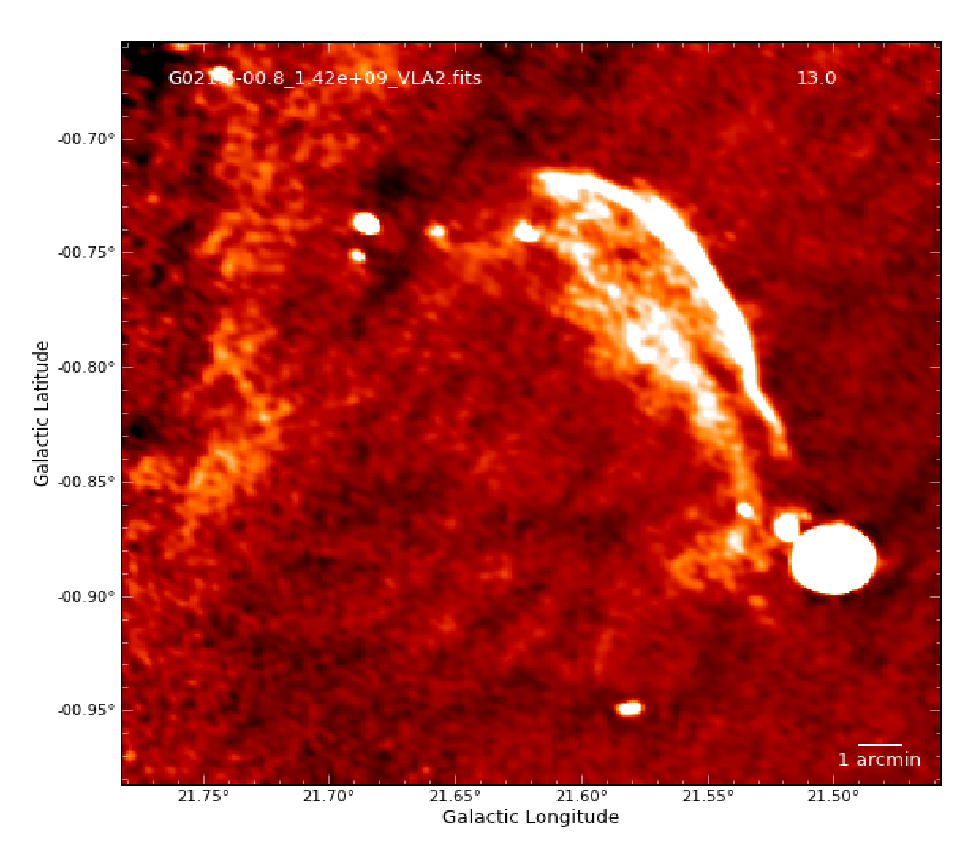
\includegraphics[width=0.325\textwidth]{G21.eps}
    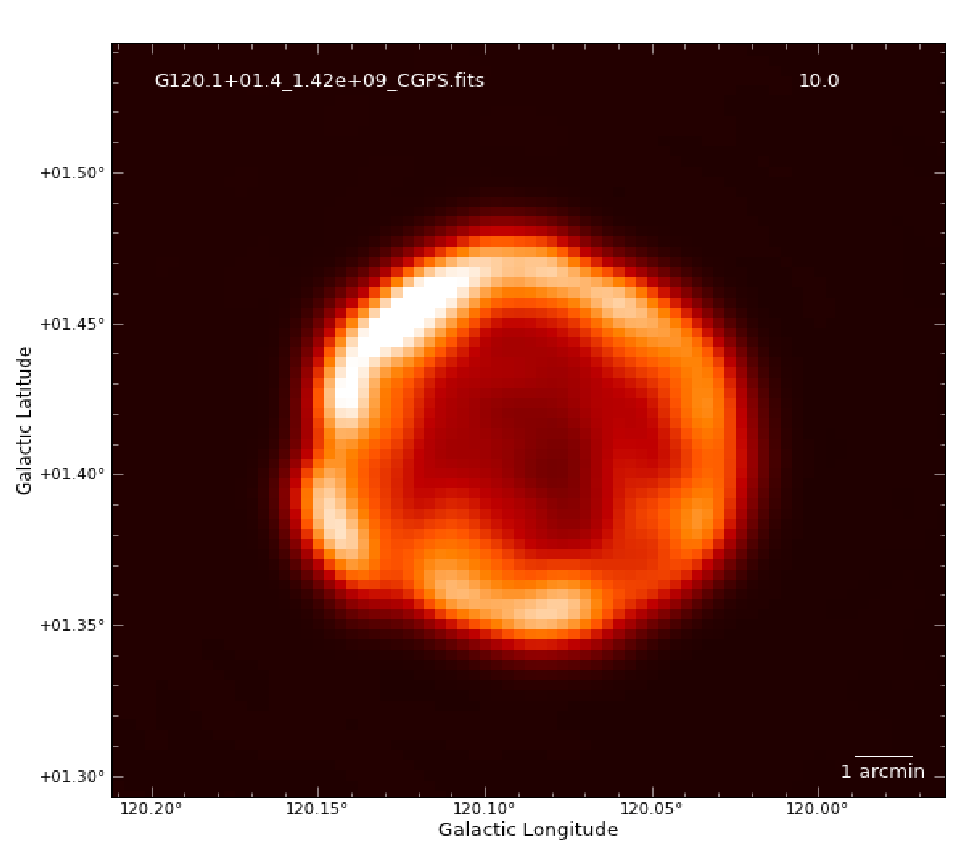
\includegraphics[width=0.325\textwidth]{G120.eps}
    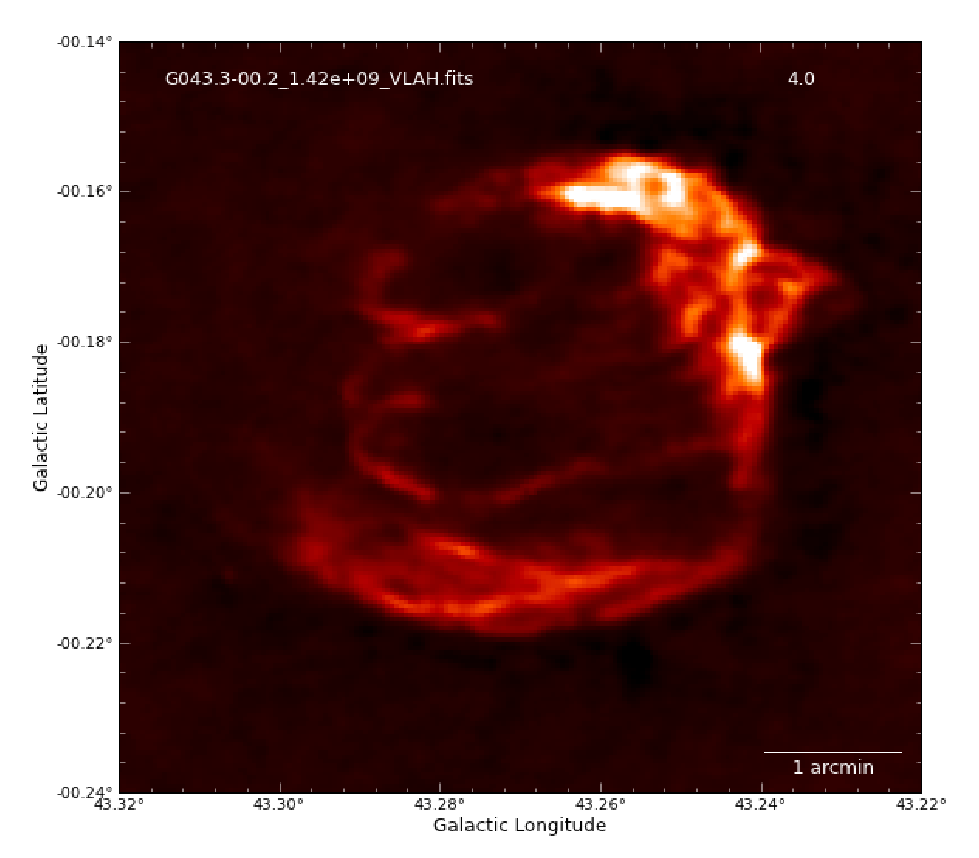
\includegraphics[width=0.325\textwidth]{G43.eps}
    \caption{典型的多层、环形、不规则遗迹: G21.6-0.8,G120.1+1.4和G43.3-0.2。 }
\label{fig:stat}
\end{figure*}

\begin{table*}
  \caption{七类遗迹的统计}
  \label{table:stat}
  \centering
  \begin{tabular}{l l l}
      \hline\hline
      类型                           & 数量           & 样本               \\
      \hline
      单边小弧度         & 35                &G4.2-3.5, G5.9+3.1, G6.1+0.5, G6.4+4.0, G7.0-0.1, \\& & G7.2+0.2,
      G11.1+0.1, G11.1-0.7, G12.2+0.3,\\& &  G14.3+0.1, G17.4-0.1, G24.7-0.6, G49.2-0.7, G57.2+0.8,\\& & G59.8+1.2, G65.1+0.6,
      G310.8-0.4, G327.4+1.0, G338.1+0.4,\\& & G348.5-0.0, G348.7+0.3, G350.0-2.0, G351.7+0.8, G351.9-0.9,\\& &  G354.1+0.1,
      G359.0-0.9\\
      \hline
      单边大弧度         & 15                &G0.0+0.0, G1.9+0.3, G3.8+0.3, G8.3-0.0, G9.8+0.6,\\& & G18.6-0.2,
      G18.8+0.3, G33.2-0.6,  G55.7+3.4, G66.0-0.0,\\& & G116.9+0.2, G119.5+10.2, G298.6-0.0, G321.9-1.1, G342.1+0.9\\
      \hline
      双边对称             & 17                &G0.9+0.1, G1.0-0.1, G3.7-0.2, G8.7-5.0, G16.2-2.7,\\& & G21.0-0.4,
      G23.3-0.3,  G36.6+2.6,  G59.5+0.1,  G65.3+5.7, \\& & G296.5+10.0, G321.9-0.3, G327.6+14.6, G332.0+0.2, G349.2-0.1,
      \\& & G353.9-2.0, G356.3-1.5\\
      \hline
      八字形            & 11                &G11.0-0.0, G21.8-0.6, G29.7-0.3, G42.8+0.6, G53.6-2.2, \\& & G54.4-0.3,
      G64.5+0.9,  G304.6+0.1, G348.5+0.1, G350.1-0.3, \\& & G352.7-0.1\\
      \hline
      多层                     & 13                &G21.6-0.8, G24.7+0.6, G46.8-0.3, G85.4+0.7, G93.3+6.9, \\& & G109.1-1.0,
       G284.3-1.8,  G286.5-1.2,  G318.9+0.4, G320.6-1.6,\\& & G327.4+0.4, G358.1+1.0, G358.5-0.9\\
      \hline
      环形                        & 42                &G4.5+6.8, G5.2-2.6, G6.5-0.4, G11.2-0.3, G11.4-0.1, \\& & G15.9+0.2,
      G16.7+0.1, G18.1-0.1,  G21.5-0.9,  G27.4+0.0,\\& & G69.7+1.0, G82.2+5.3, G83.0-0.3, G84.2-0.8, G111.7-2.1,\\& & G120.1+1.4,
      G132.7+1.3,  G179.0+2.6, G180.0-1.7, G184.6-5.8,\\& & G261.9+5.5, G290.1-0.8,  G299.2-2.9, G301.4-1.0, G302.3+0.7,
      \\& & G308.1-0.7, G310.6-0.3, G311.5-0.3, G315.4-2.3,  G322.5-0.1,\\& & G326.3-1.8, G327.1-1.1, G327.2-0.1,  G332.4-0.4,
      G337.3+1.0, \\& & G346.6-0.2,  G354.8-0.8, G355.6-0.0, G355.9-2.5, G356.2+4.5,\\& & G358.0+3.8, G359.1-0.5\\
      \hline
      不规则                       & 155               &\\
      \hline
  \end{tabular}\\
\end{table*}

根据\citet{West2016}收集的超新星遗迹射电图像,我们根据其射电形态把遗迹分为七类:单边
小弧度、单边大弧度、双边对称、八字形、多层、环形、不规则遗迹。
其中多层遗迹定义为其一边或双边有两层或者多层壳层。
比较典型的多层、环形、不规则遗迹见图~\ref{fig:stat},这七类遗迹的统计结果见
表~\ref{table:stat}。
我们只统计了288个遗迹,因为其它遗迹的图像很模糊,无法辨别。
因为不规则类型遗迹很多,我们只列出了除不规则遗迹外的其它类型遗迹的样本。

\subsection{垂直事例}

\begin{figure*}
    \centering
    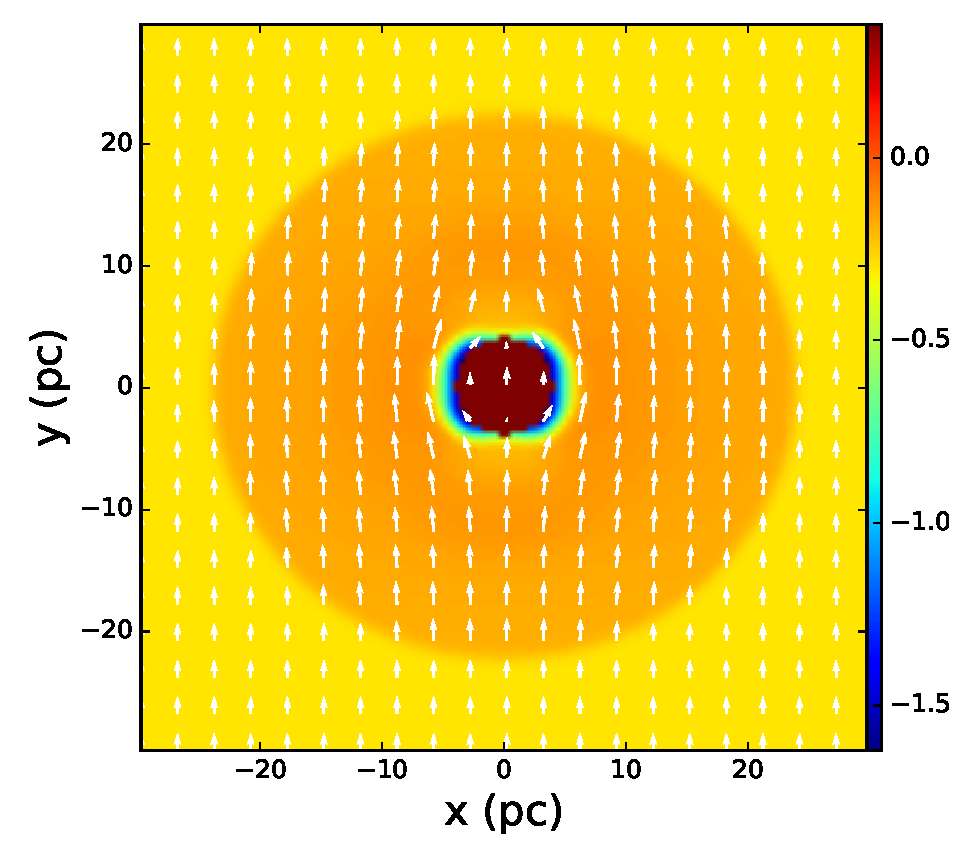
\includegraphics[width=0.325\textwidth]{rho_t0_density1_E1_xyp.eps}
    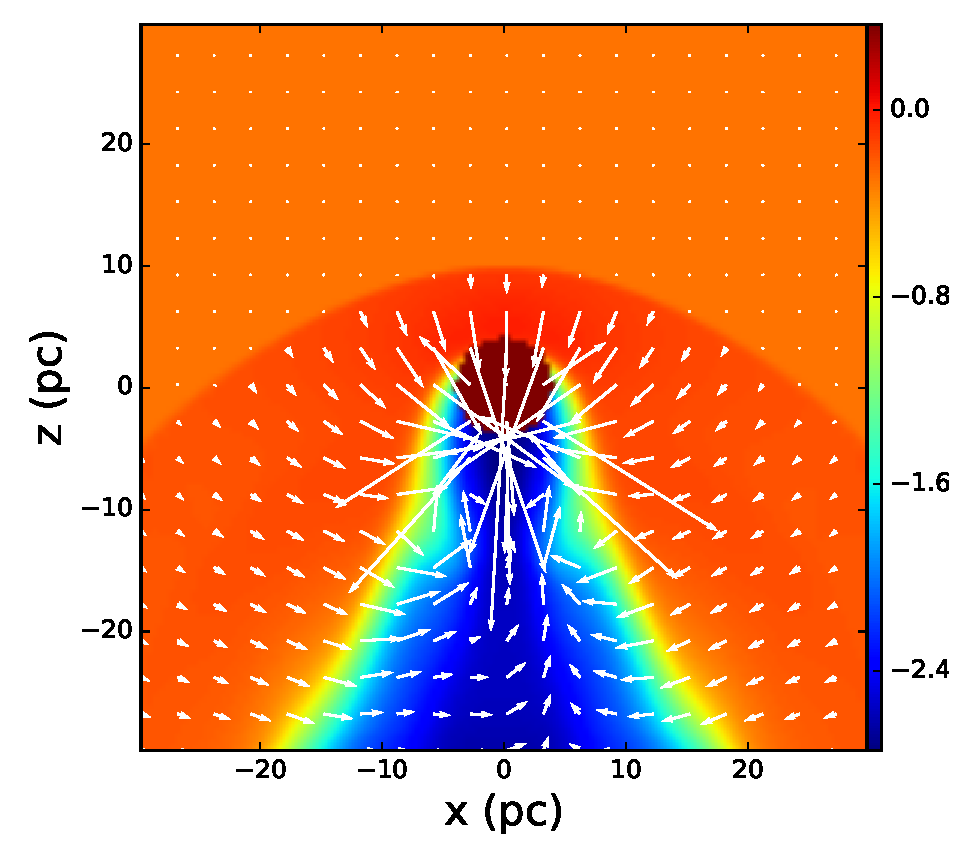
\includegraphics[width=0.325\textwidth]{rho_t0_density1_E1_xzp.eps}
    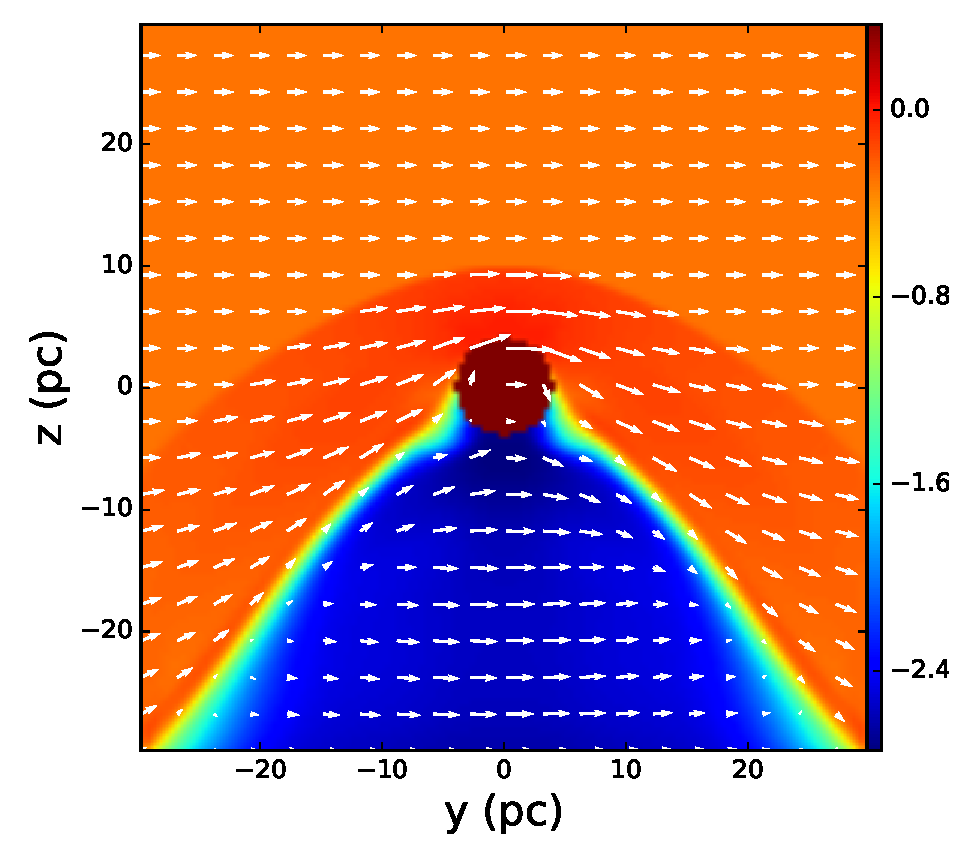
\includegraphics[width=0.325\textwidth]{rho_t0_density1_E1_yzp.eps}\newline
    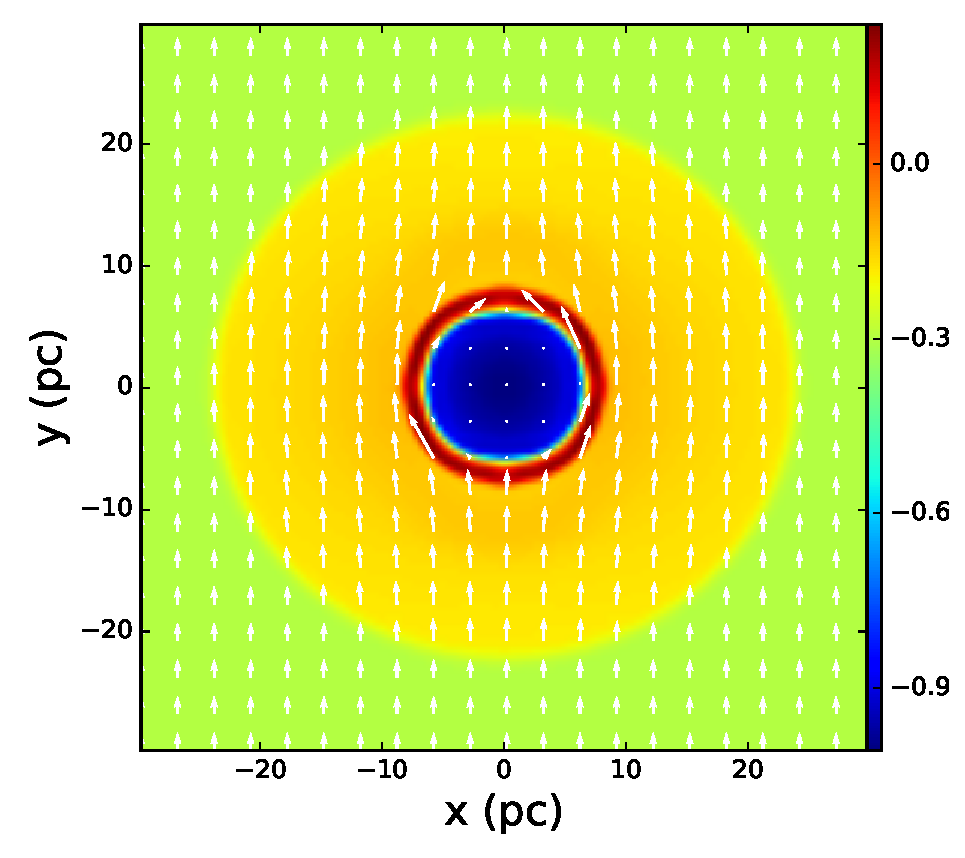
\includegraphics[width=0.325\textwidth]{rho_t6_density1_E1_xyp.eps}
    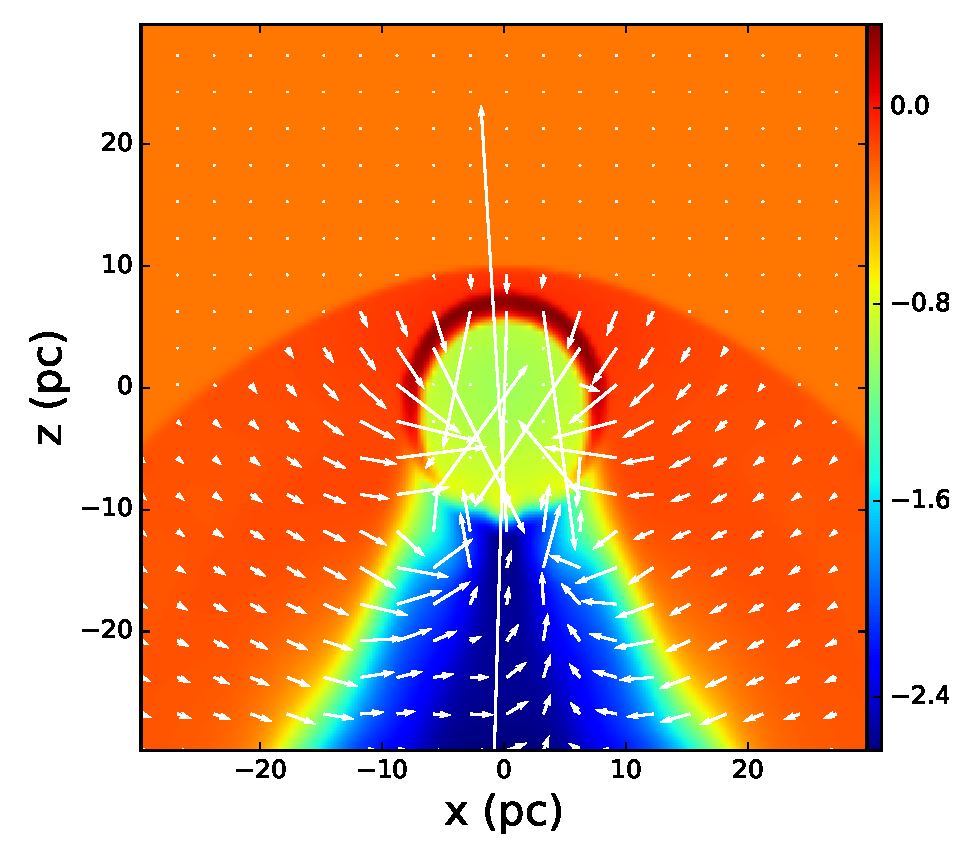
\includegraphics[width=0.325\textwidth]{rho_t6_density1_E1_xzp.eps}
    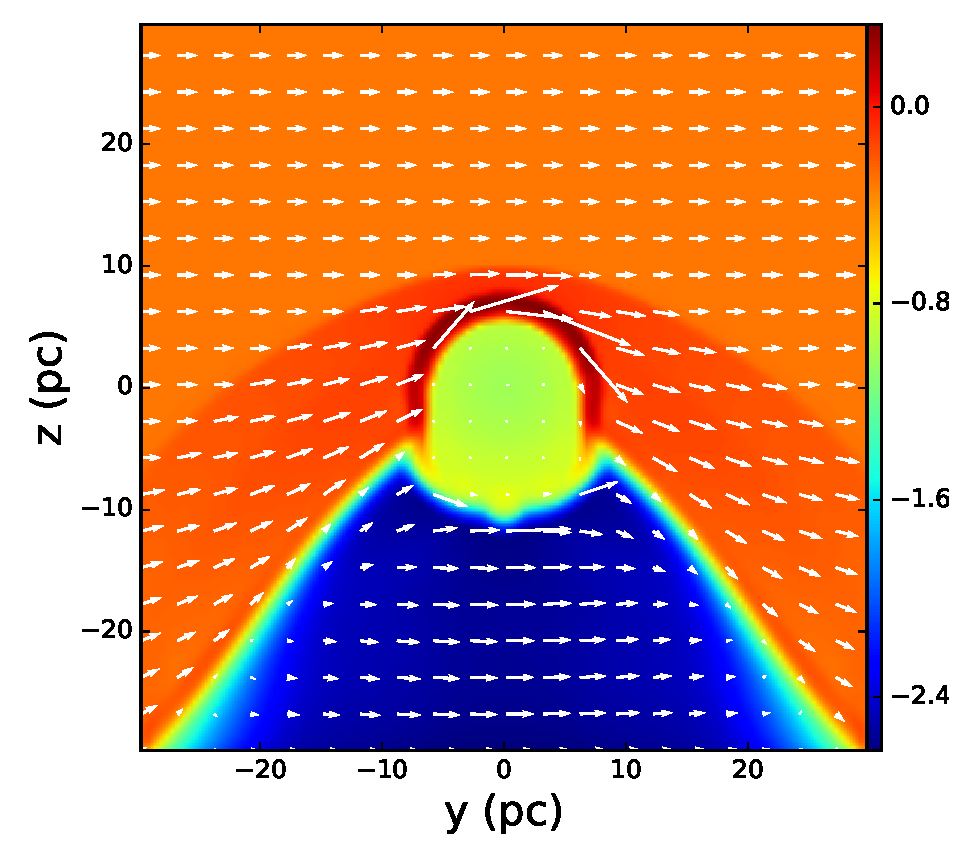
\includegraphics[width=0.325\textwidth]{rho_t6_density1_E1_yzp.eps}\newline
    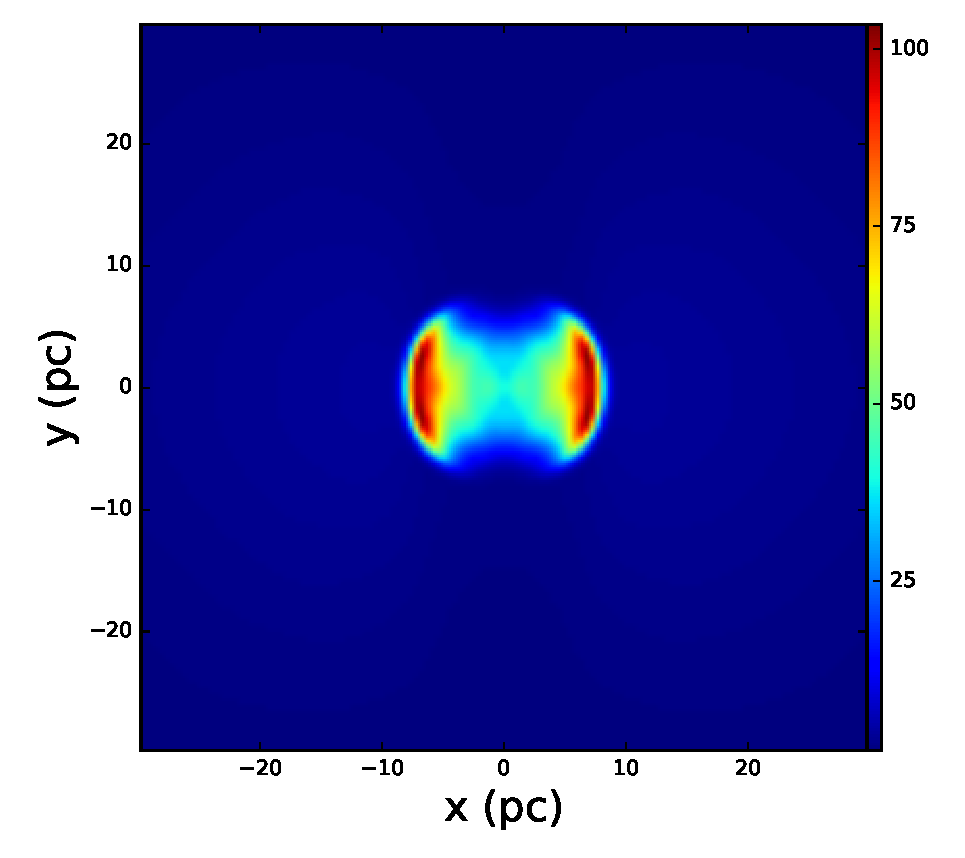
\includegraphics[width=0.325\textwidth]{t6_xyp.eps}
    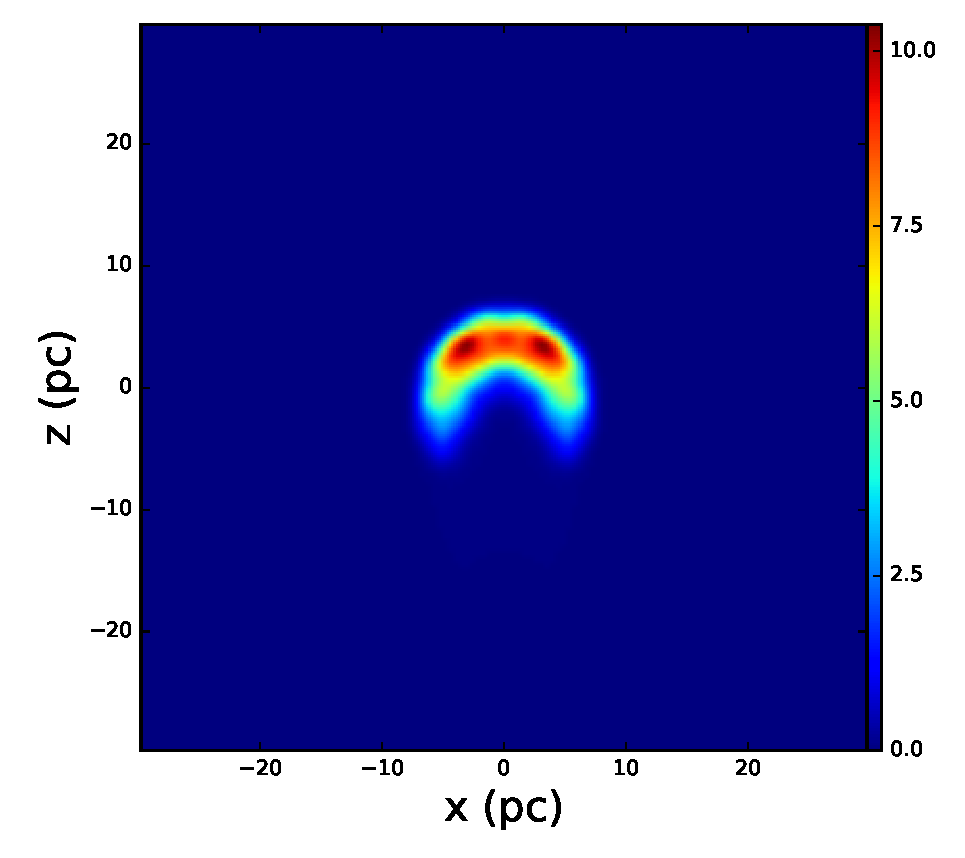
\includegraphics[width=0.325\textwidth]{t6_xzp.eps}
    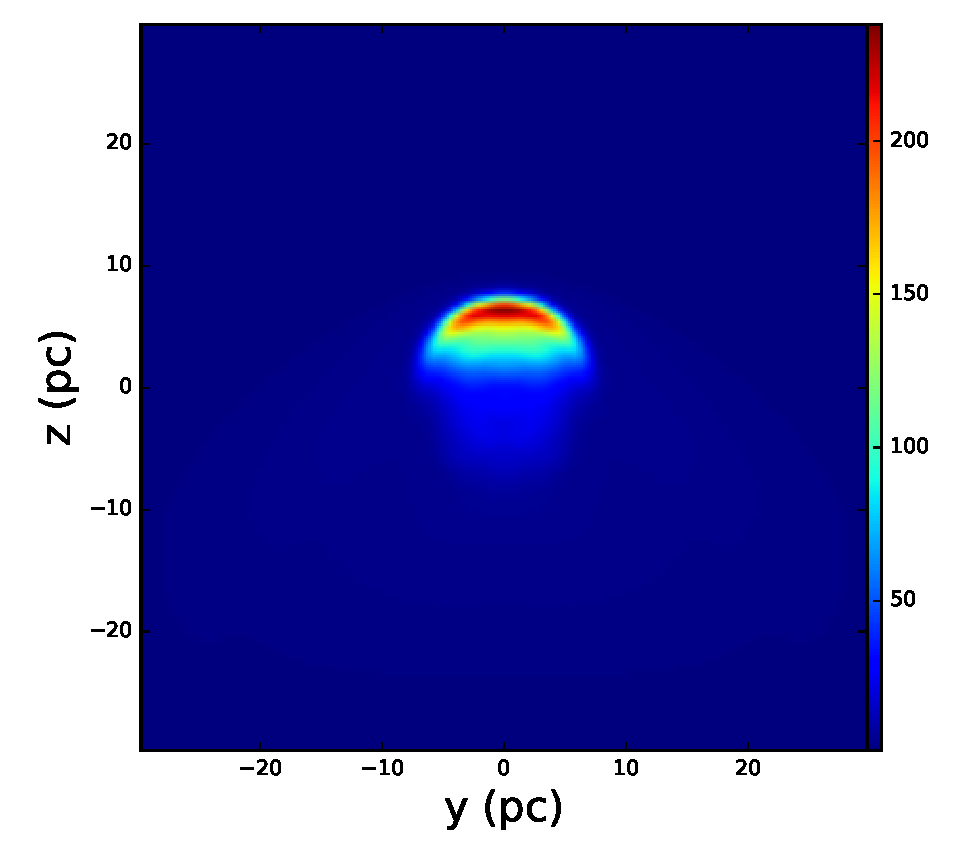
\includegraphics[width=0.325\textwidth]{t6_yzp.eps}\newline
    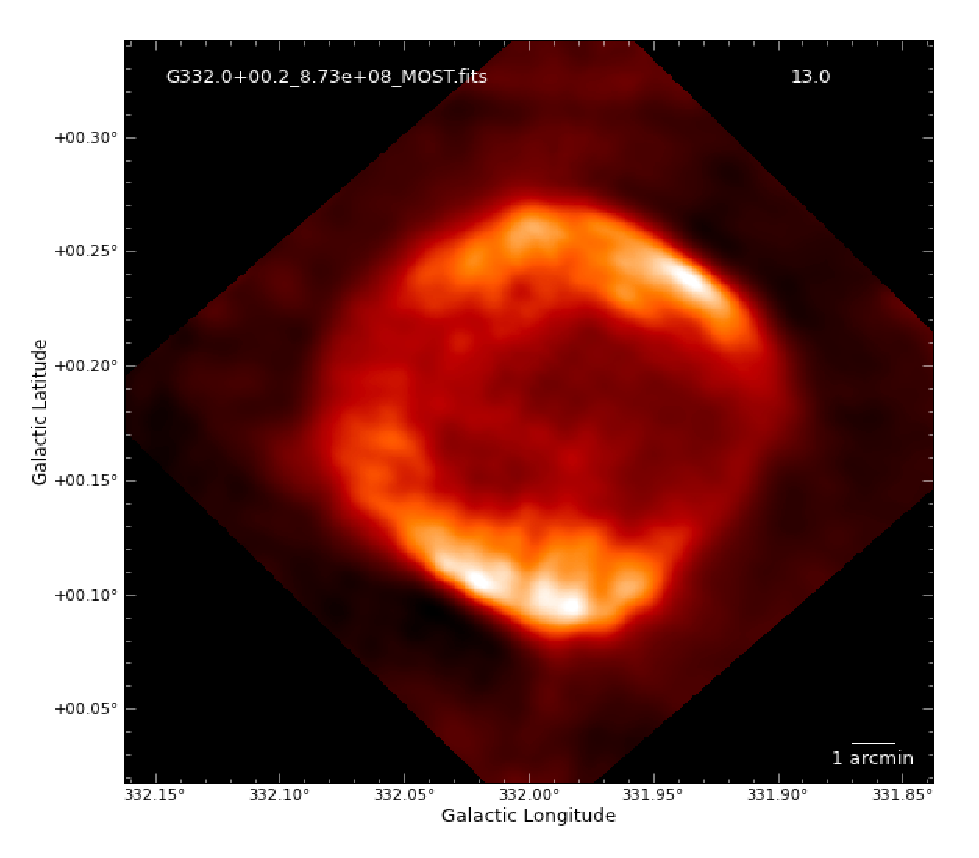
\includegraphics[width=0.325\textwidth]{G332.eps}
    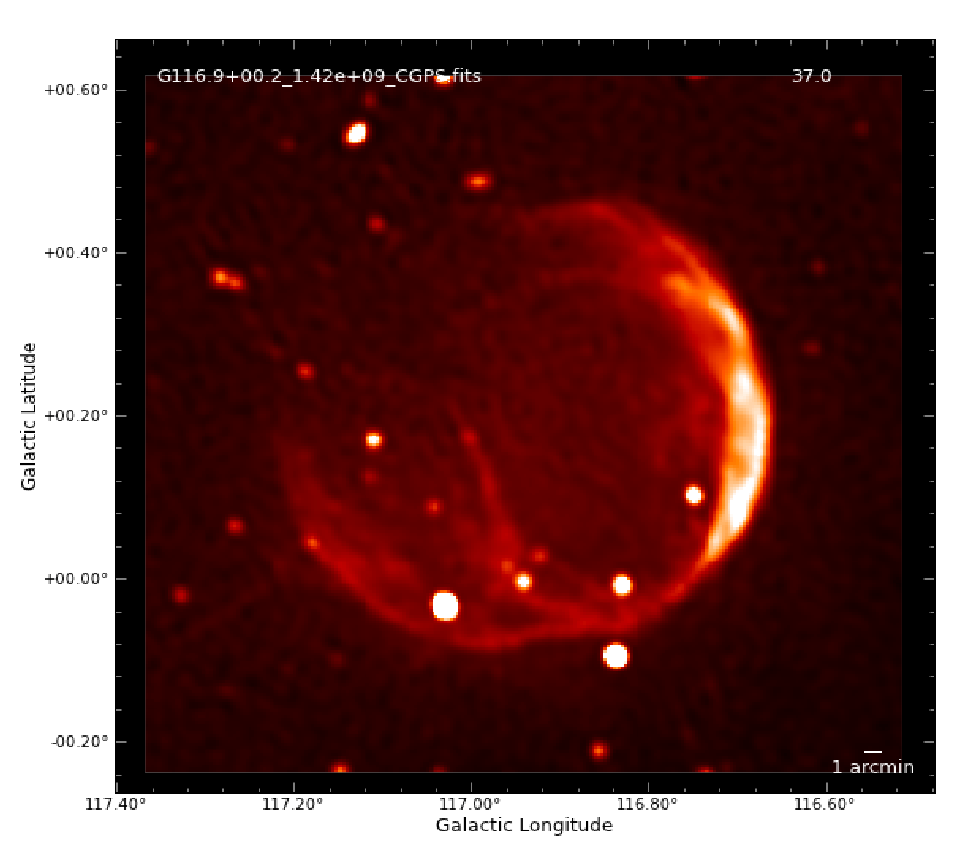
\includegraphics[width=0.325\textwidth]{G116.eps}
    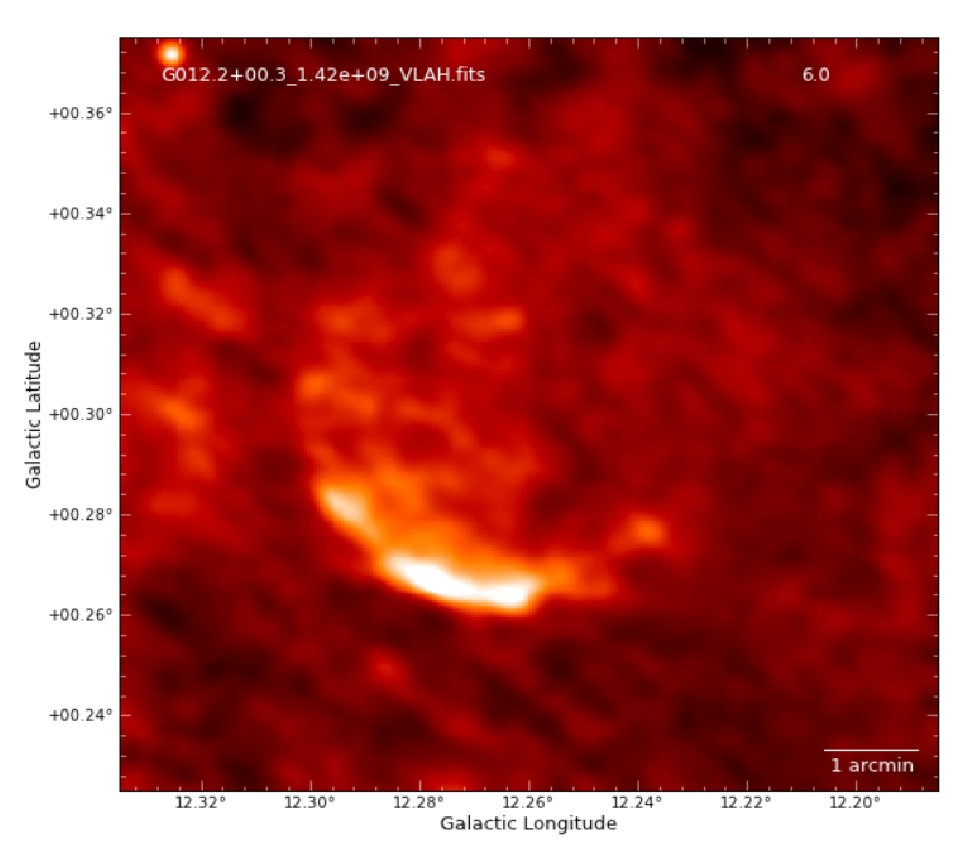
\includegraphics[width=0.325\textwidth]{G12.eps}
    \caption{垂直事例的模拟图像以及对应的真实射电图像。 顶部三幅图是从不同方向看去的星风
    模拟结果。第二行是以顶部的星风模拟结果为初始条件的超新星遗迹模拟结果。第三行是从第二行
    的模拟结果转化而来的相对射电密度图像。最后一行是与模拟的射电形态相似的实际观测到的遗迹
    G332.0+0.2,G116.9+0.2和G12.2+0.3\citep{West2016}。这三个遗迹分别分类为双边对称、
    单边大弧度和单边小弧度遗迹。上面两行的彩色背景是单位为log(cm$^{-3}$)的密度分布,箭头
    的长度和方向分别代表磁场强度和方向。}
\label{fig:per}
\end{figure*}

垂直事例的模拟结果见图~\ref{fig:per}。
顶部的三幅图就是遗迹模拟的初始条件,其中包括两部分,一部分是周围介质分布,一部分是中间
后来加上去的超新星爆发区域。
周围介质分布其实是之前星风模拟的结果,直接作为遗迹模拟的初始条件,而超新星爆发区域是直接
通过解析解计算得来。
而星风模拟的初始条件是假设磁场沿着y轴方向,前身星速度沿着z轴方向,这导致我们在y-z平面
能看到明显的弓形结构,在x-z平面能看到磁场非常混乱。
为了看得更清晰,不同图像的箭头和颜色使用不同的标度,也就不能通过箭头长度和颜色变化对比
不同图像的相应参数。
但是标注的数值是绝对的,可以用来比较不同图像的密度。

\begin{figure}
    \centering
    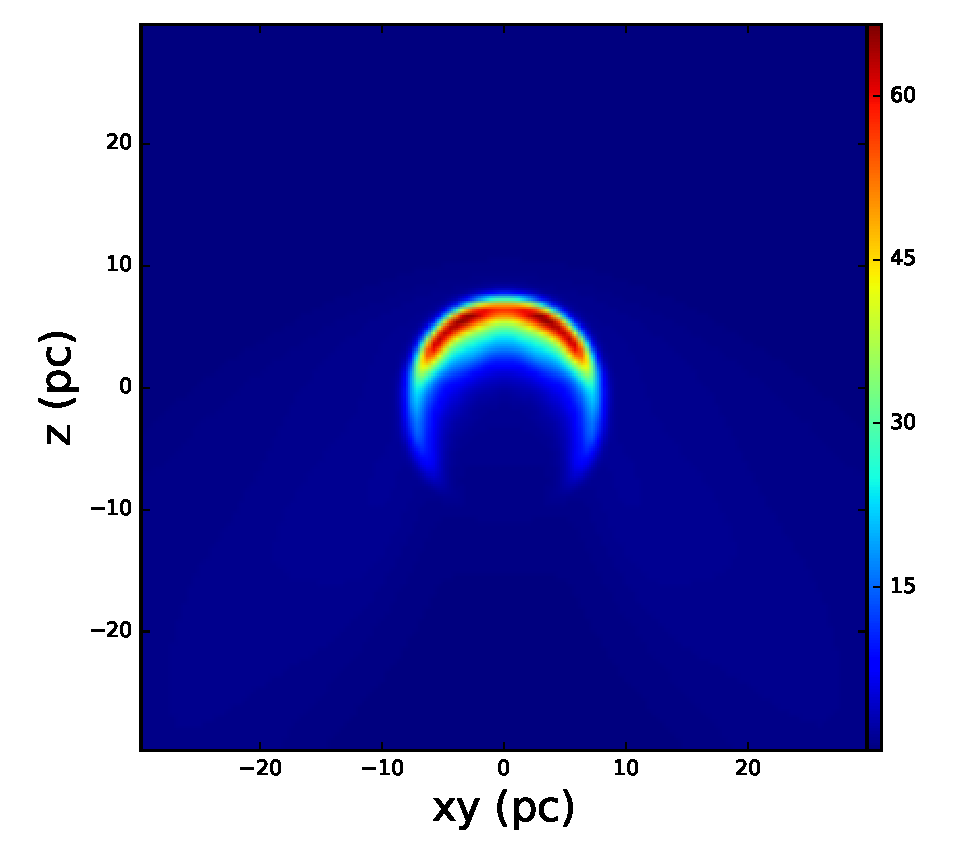
\includegraphics[width=0.4\textwidth]{t6_xzp_45deg.eps}
    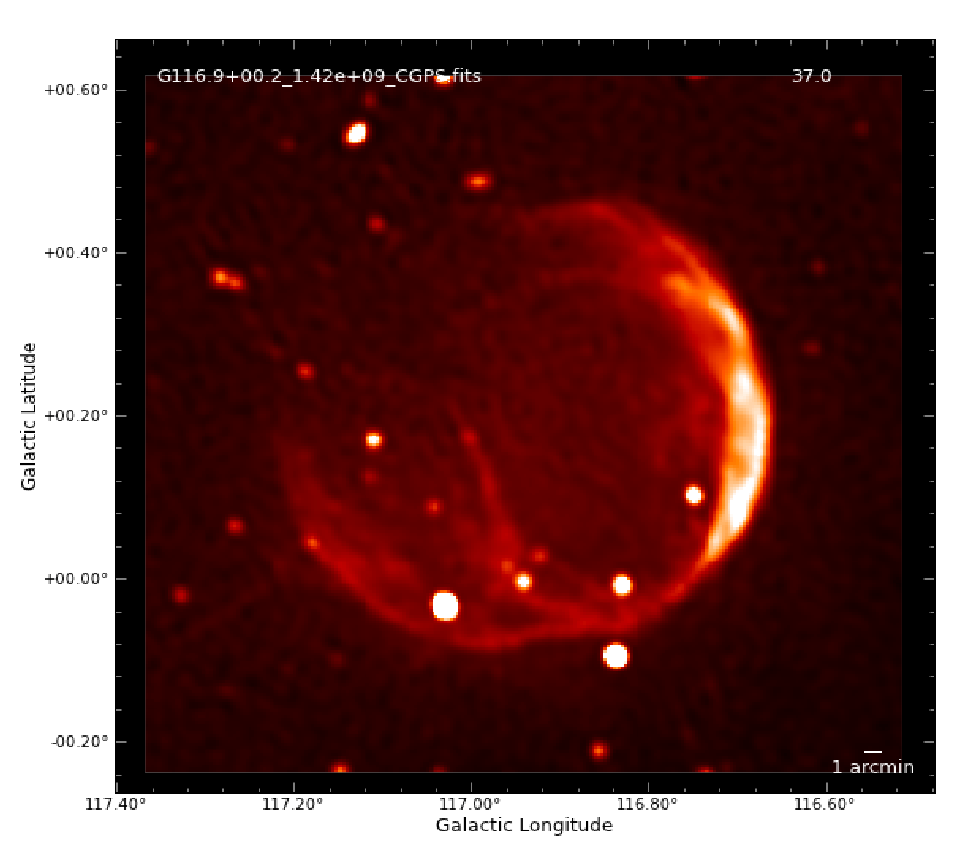
\includegraphics[width=0.4\textwidth]{G116.eps}
    \caption{沿着z轴旋转$45\degr$后的模拟射电图像和G116.9+0.2的真实观测到的射电图像
    \citep{West2016,Tian2006}。}
\label{fig:45deg}
\end{figure}

\begin{figure*}
    \centering
    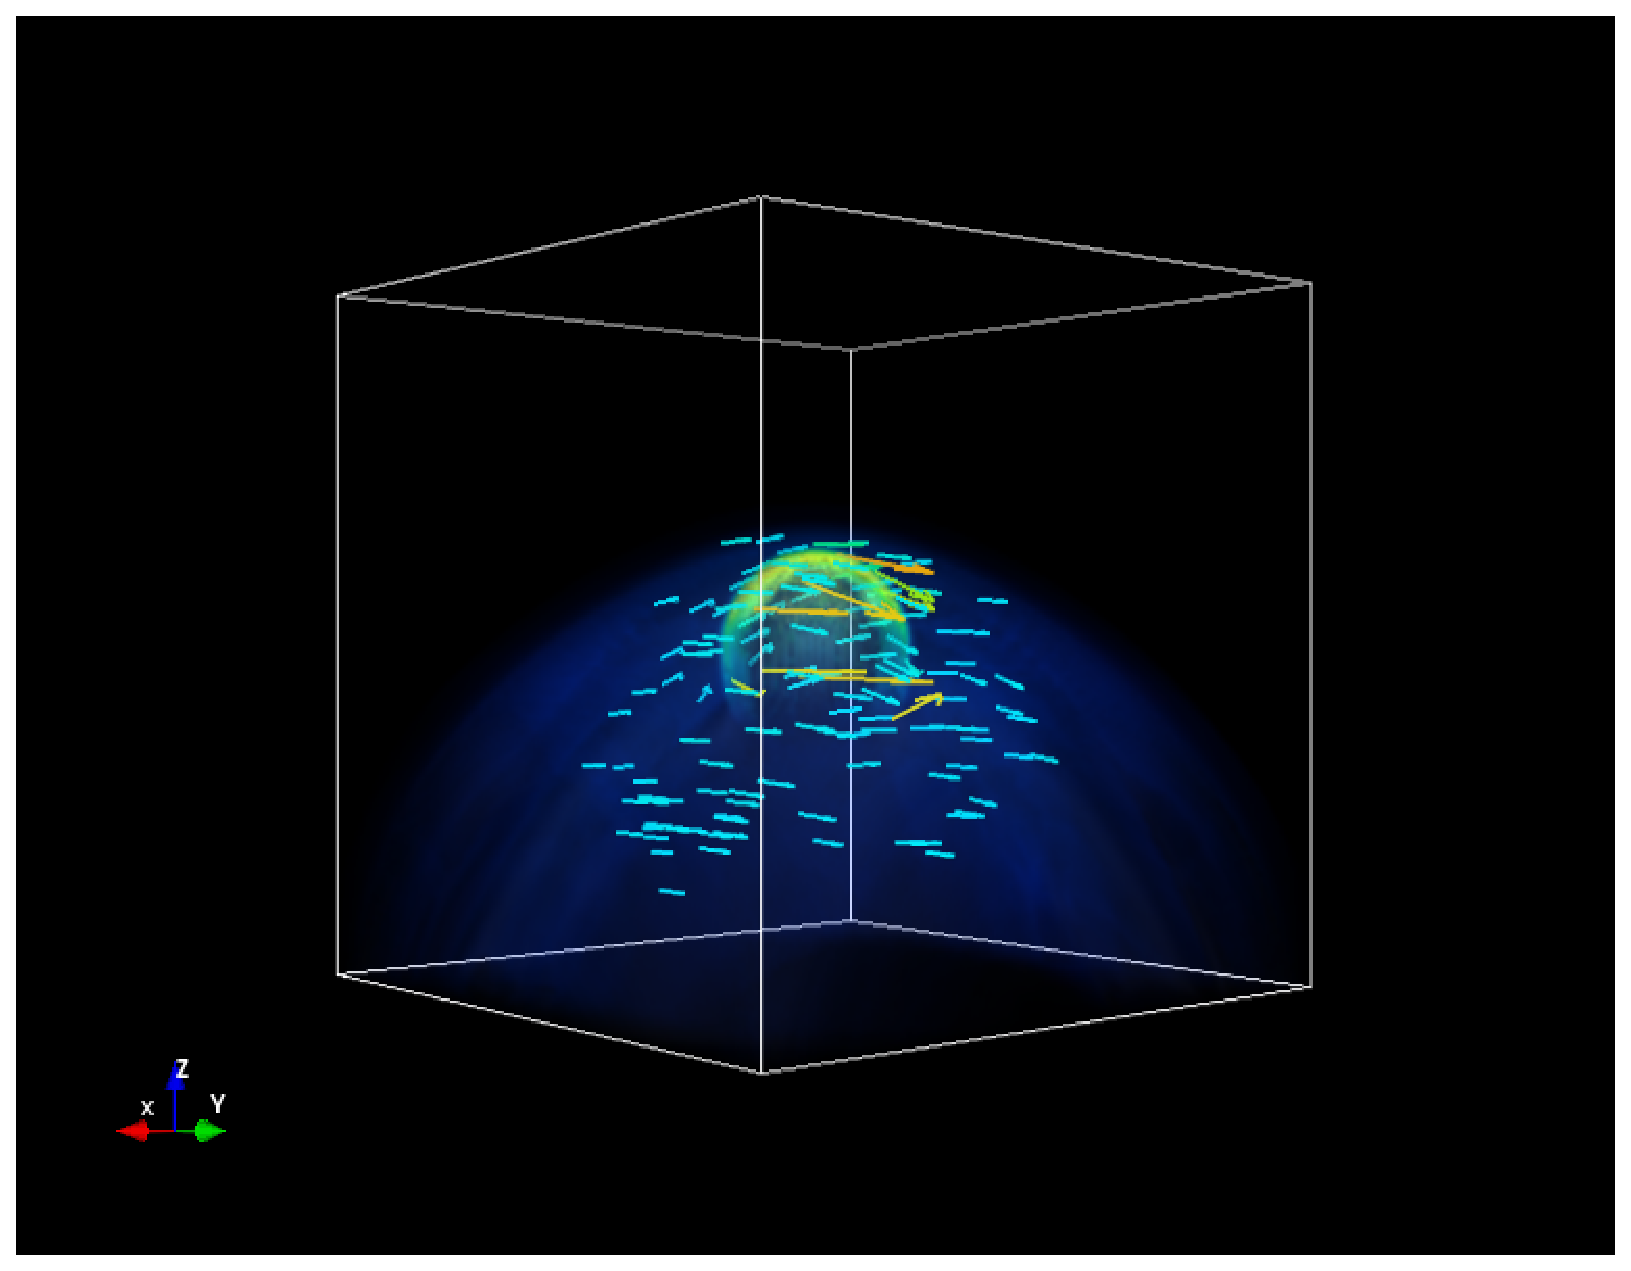
\includegraphics[width=0.9\textwidth]{3D.eps}
    \caption{从x-z平面沿着z轴旋转$50\degr$后模拟的三维图。如果转$45\degr$, 中间两条
    垂直的线就重合了,透视效果很差,所以我们转了$50\degr$。彩色的背景是相对射电流量密度,
    箭头代表磁场,越黄的颜色数值越大。(这个图在发表文章的线上版本中是动态图。)}
\label{fig:3D}
\end{figure*}

\begin{figure*}
    \centering
    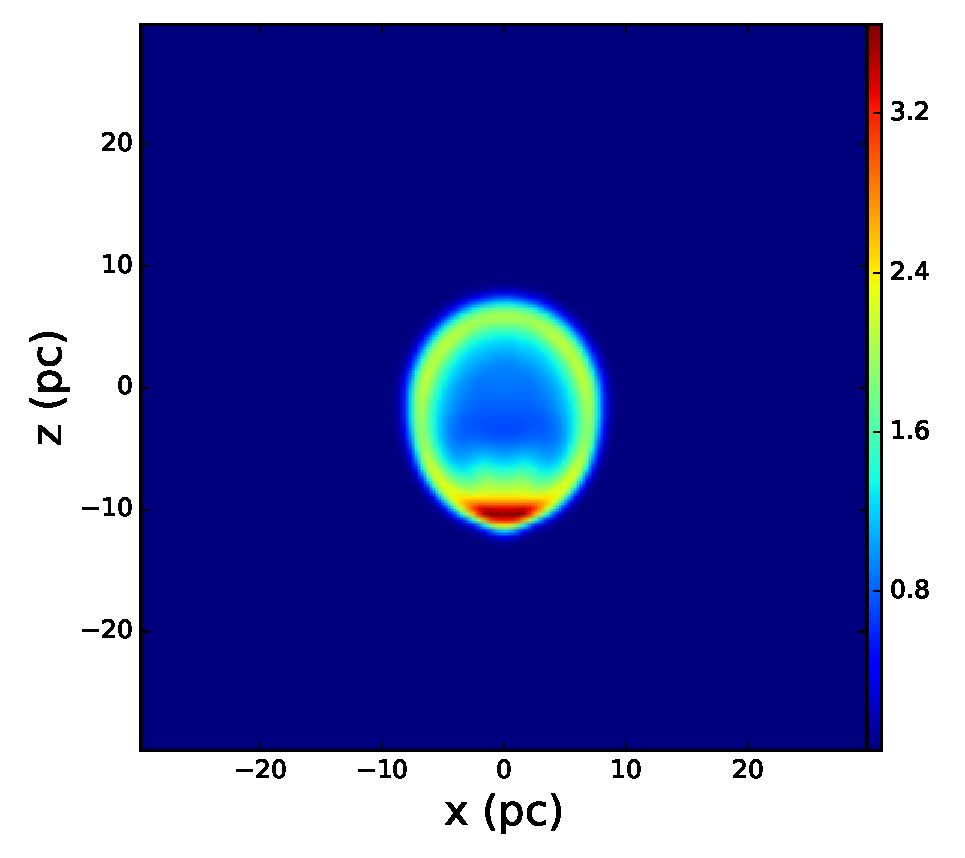
\includegraphics[width=0.45\textwidth]{T.eps}
    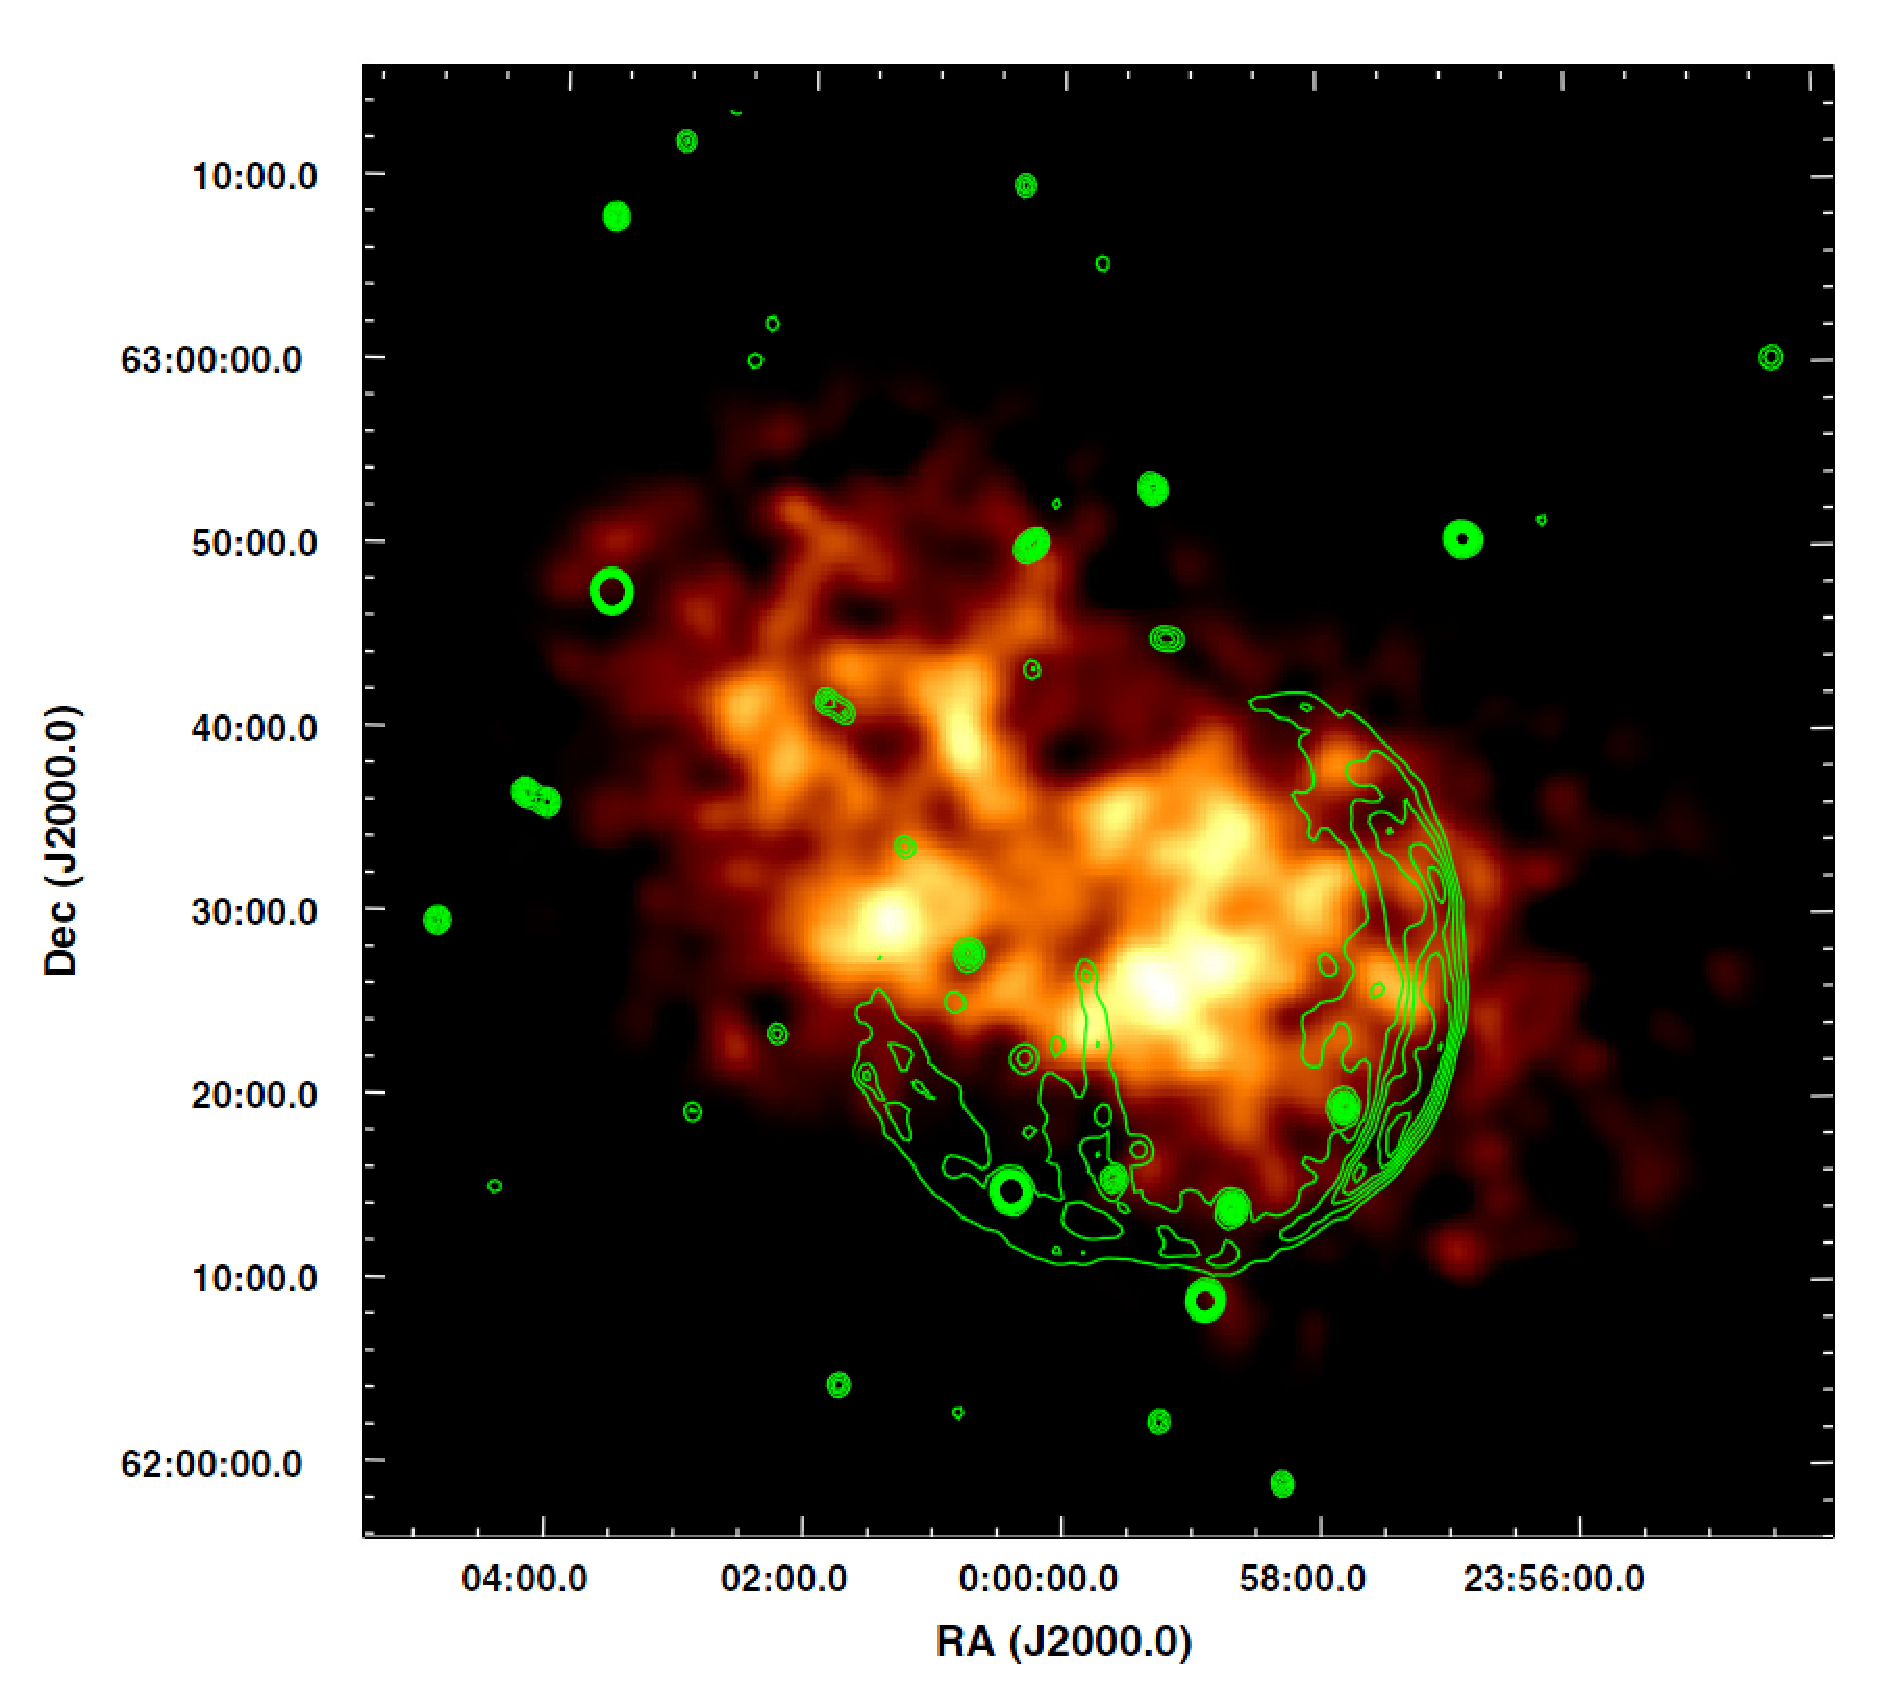
\includegraphics[width=0.45\textwidth]{xx.eps}
    \caption{\textit{左图:}x-z平面的相对温度分布。\textit{右图:} ASCA (Advanced Satellite for
    Cosmology and Astrophysics)望远镜观测到的G116.9+0.2的X图像G116.9+0.2,外加CGPS
     (Canadian Galactic Plane Survey)巡天的射电图像等高线\citep{Pannuti2010}。}
\label{fig:X}
\end{figure*}

图~\ref{fig:per}的第二行展示了模拟开始1200年后的结果,如果加上初始的650年,这个虚拟
遗迹的真实年龄是1850年。
图~\ref{fig:per}的第三行展示了转化为射电流量密度的模拟图像,这个结果是有点令人吃惊的。
这一个模拟结果,从不同方向来看,可以得到三个不同类型的遗迹:双边对称、单边大弧度和单边
小弧度遗迹。
作为比较,我们在图~\ref{fig:per}的最后一行展示了相应类型的三幅真实遗迹的射电图像。
这说明,这三类遗迹可以来源于同一个前身星,它们的形态取决于看它们的方向。
而在之前,我们只对双边对称遗迹有较好的模拟、观测研究\citep{Gaensler1999,Petruk2009a},
对另外两类知之甚少。
此外,我们只是展示了从三个方向看的结果,可是实际上,遗迹的形态稍微偏转角度看就会变化明显。
以超新星遗迹G116.9+0.2为例,如果沿着z轴转动$45\degr$看图~\ref{fig:per}的模拟结果,
可以在z-xy平面看到更相似的单边大弧度形态(如图~\ref{fig:45deg})。
而在偏振图上看G116.9+0.2的磁场是平行于壳层的\citep{Sun2011},这其实与本来在x-z
平面看到的结果不符。
可是,沿着z轴转动$45\degr$后,磁场方向就变得与观测相似了(如图~\ref{fig:3D})。
同时,我们注意到G116.9+0.2的X射线辐射向射电壳层反方向延展出很远\citep{Pannuti2010},
而模拟或许也可以解释这件事情(如图~\ref{fig:X})。
在图~\ref{fig:X}的左图中,下面的高温区域在图~\ref{fig:per}的第二行中图看来密度很低,
那么这里应该充满高温低密的电离气体,适合通过韧致辐射产生很强的X射线。
因此,我们猜测,或许在超新星爆发之前,前身星边运动边抛出物质,这些物质远离超新星爆发中心。
超新星爆发后,这些物质与抛射物产生的X射线一起形成了这颗遗迹奇特的X射线形态。
\citet{Craig1997,Yar-Uyaniker2004,West2016}都曾尝试解释这个X射线形态,但并没有
得出一致的结论。
如果想确定这件事,也需要更进一步的针对这颗遗迹的模拟才行。

值得一提的是,我们的模拟没有加入初始的磁场梯度或者密度梯度,即使初始介质分布是均匀的,
仍能得到各种各样的形态。
也就是说,射电形态并不仅仅依赖于初始介质分布。
因此,直接根据超新星遗迹的射电形态估算前身星形成前的没有受到星风影响的初始的磁场和密度分布,
是一件不合理的事情。
同时,也因为局部的环境会很大程度上说到前身星星风的影响,局部的磁场与银河系大尺度结构差别
很大,所以超新星遗迹的射电形态也不太适合用于推测银河系大尺度磁场和密度分布。
\citet{West2016}构建磁场模型之后,使用构建的模型模拟不同位置的超新星遗迹,并与观测比较
后验证自己模型的正确性,这种验证方式也是存在问题的。

\begin{figure*}
    \centering
    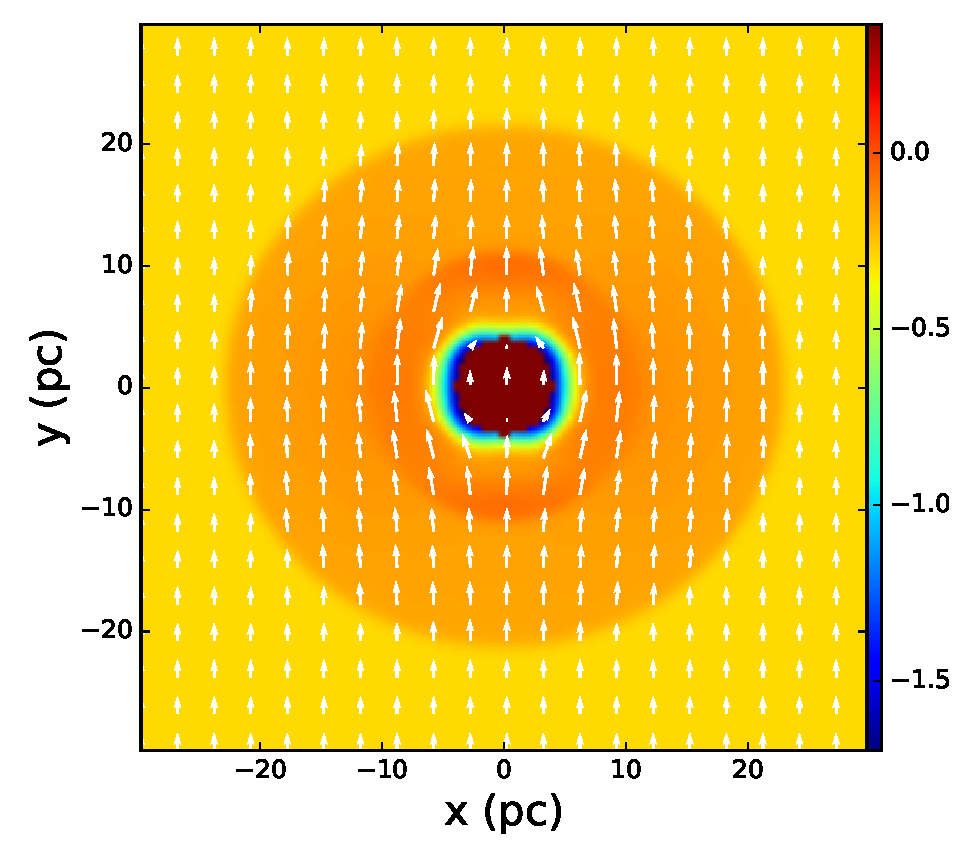
\includegraphics[width=0.325\textwidth]{rho_t0_density1_E1_xypc.eps}
    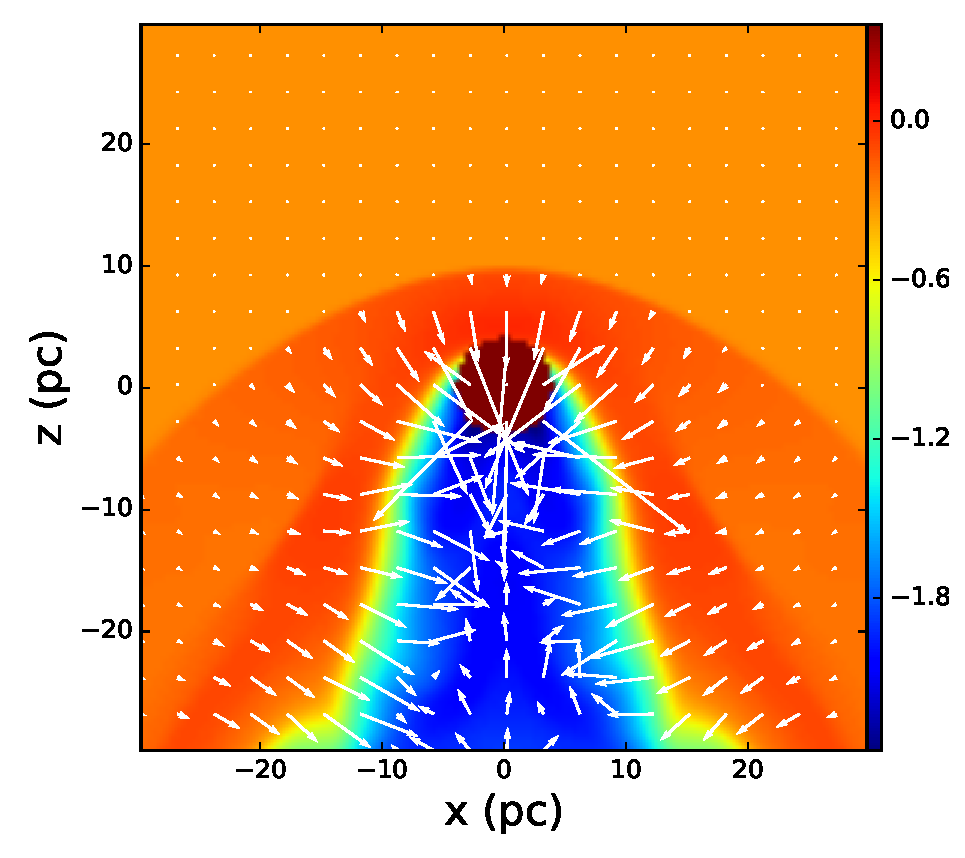
\includegraphics[width=0.325\textwidth]{rho_t0_density1_E1_xzpc.eps}
    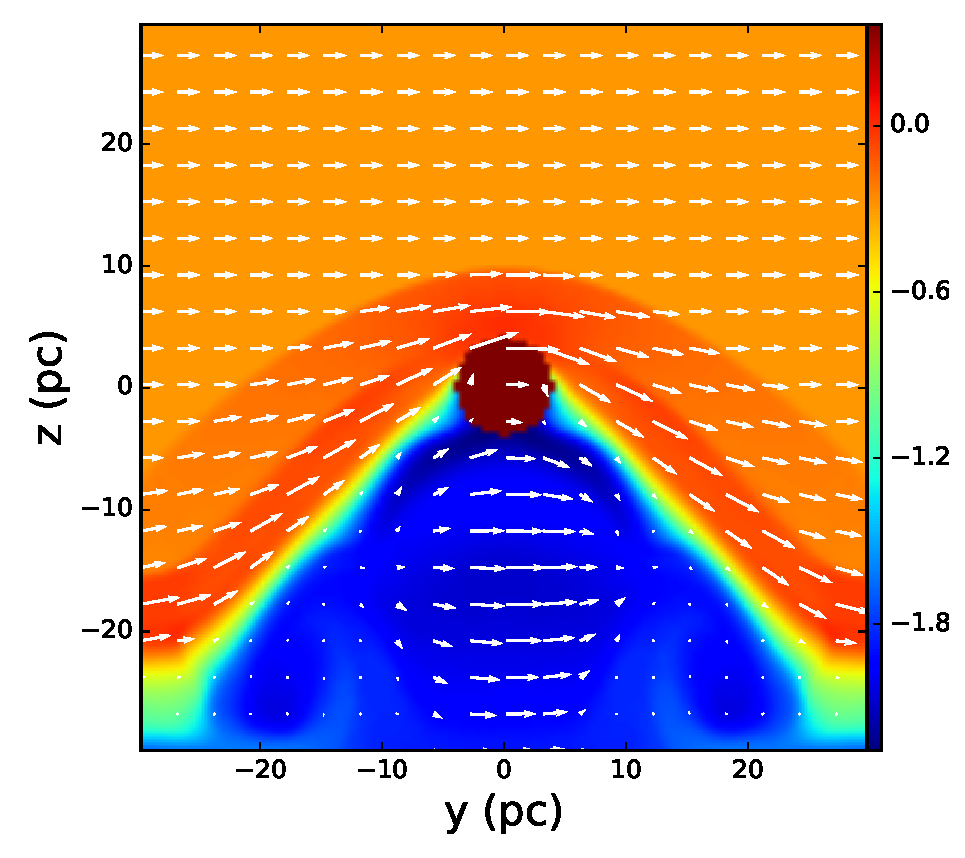
\includegraphics[width=0.325\textwidth]{rho_t0_density1_E1_yzpc.eps}\newline
    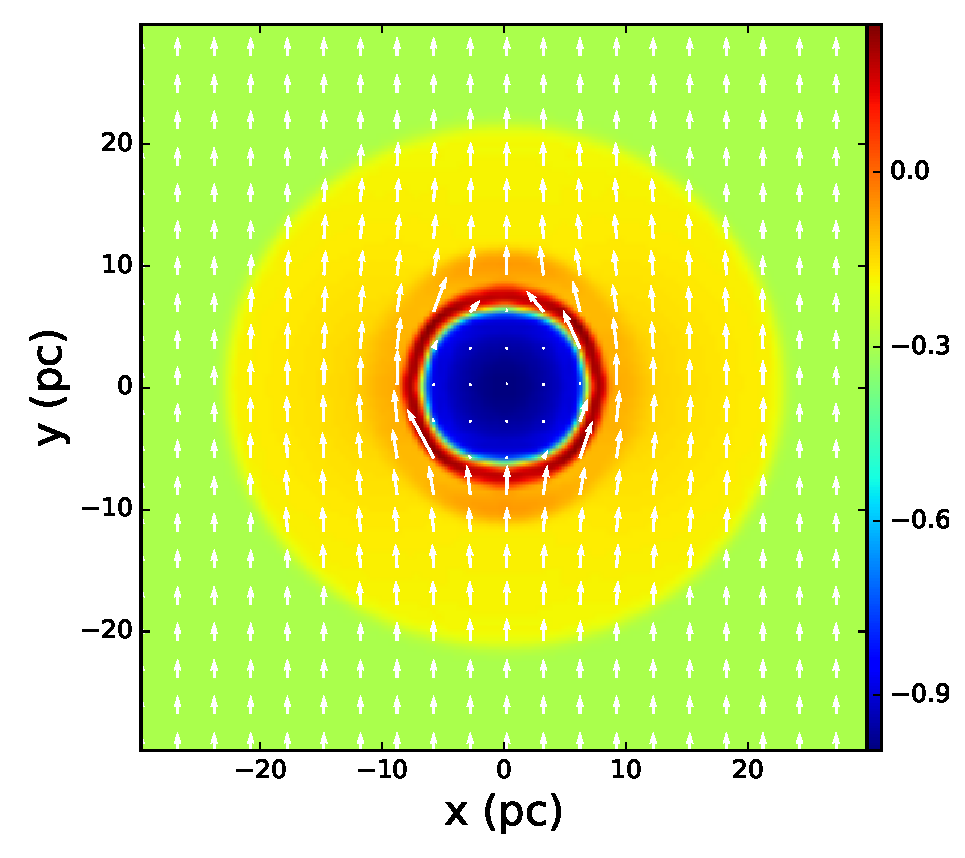
\includegraphics[width=0.325\textwidth]{rho_t6_density1_E1_xypc.eps}
    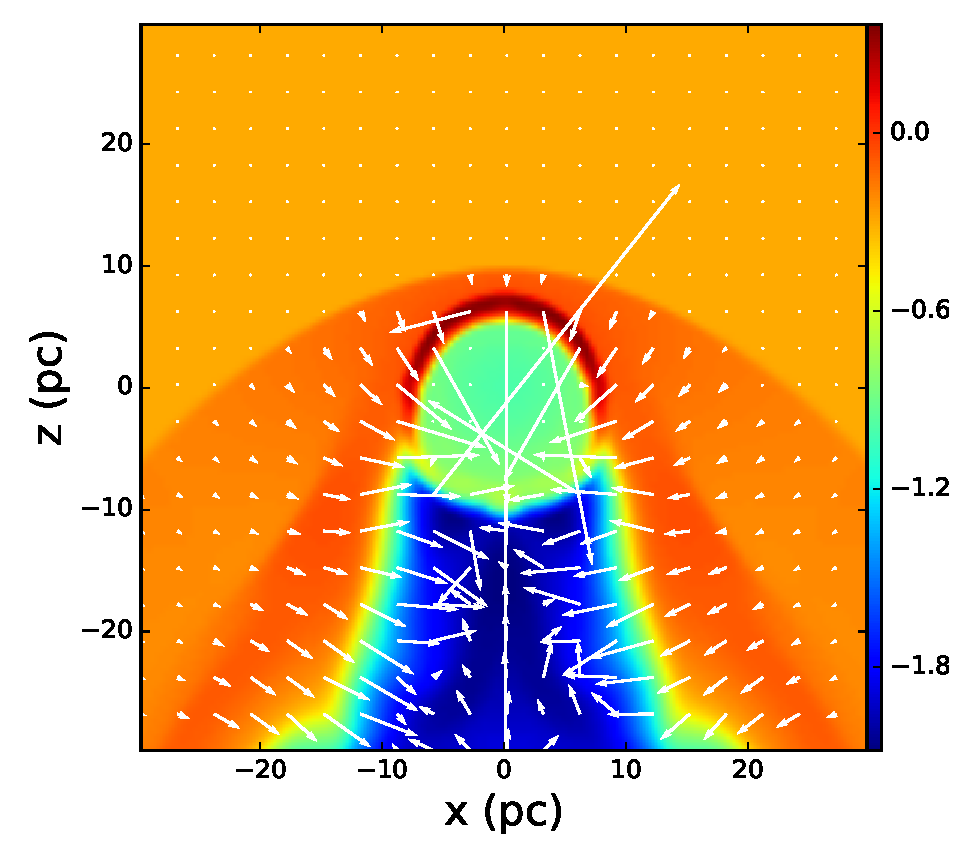
\includegraphics[width=0.325\textwidth]{rho_t6_density1_E1_xzpc.eps}
    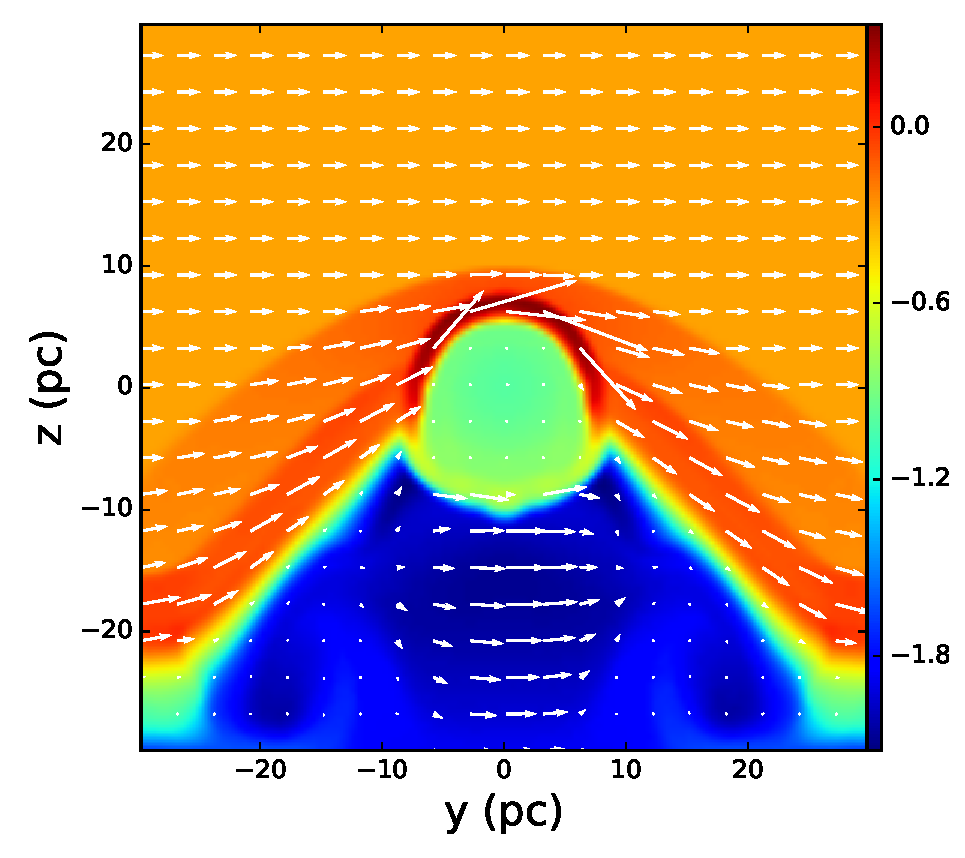
\includegraphics[width=0.325\textwidth]{rho_t6_density1_E1_yzpc.eps}\newline
    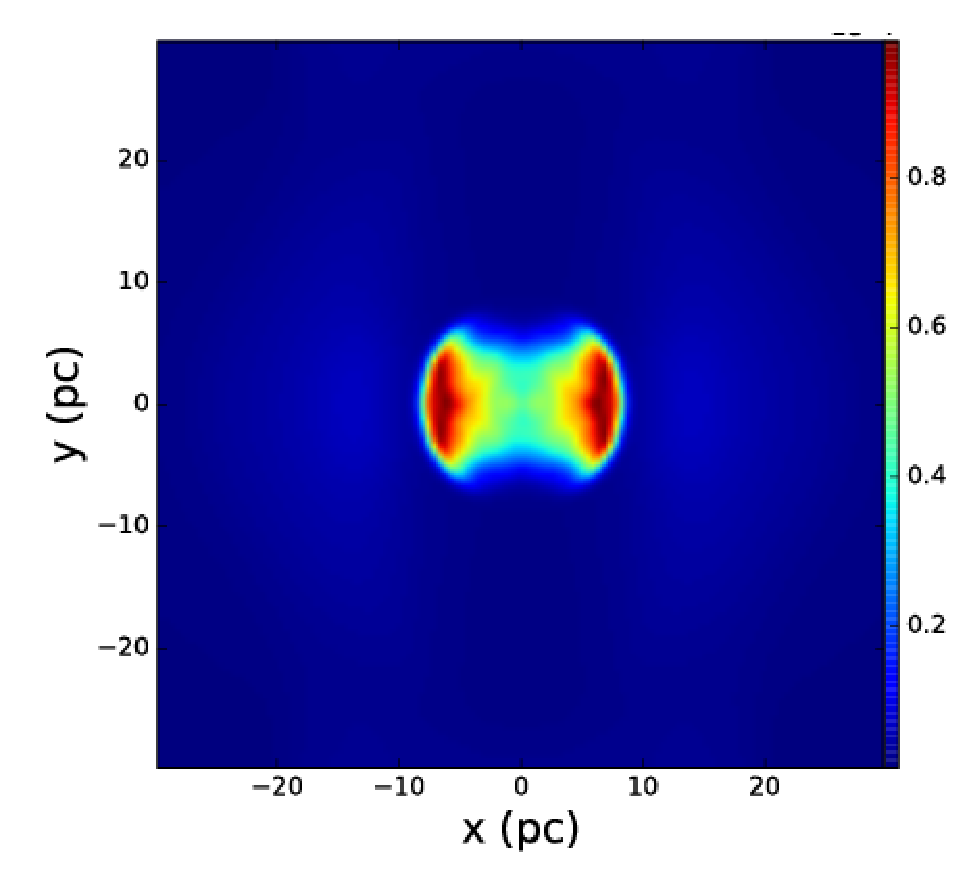
\includegraphics[width=0.325\textwidth]{t6_xypc.eps}
    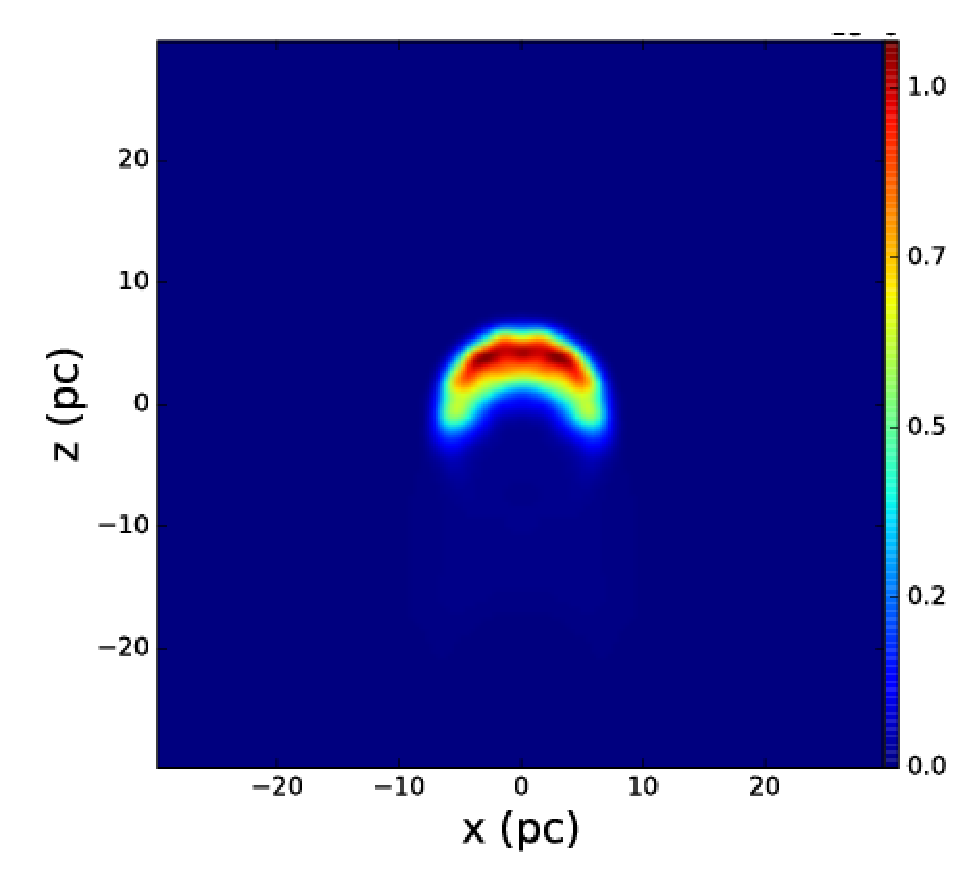
\includegraphics[width=0.325\textwidth]{t6_xzpc.eps}
    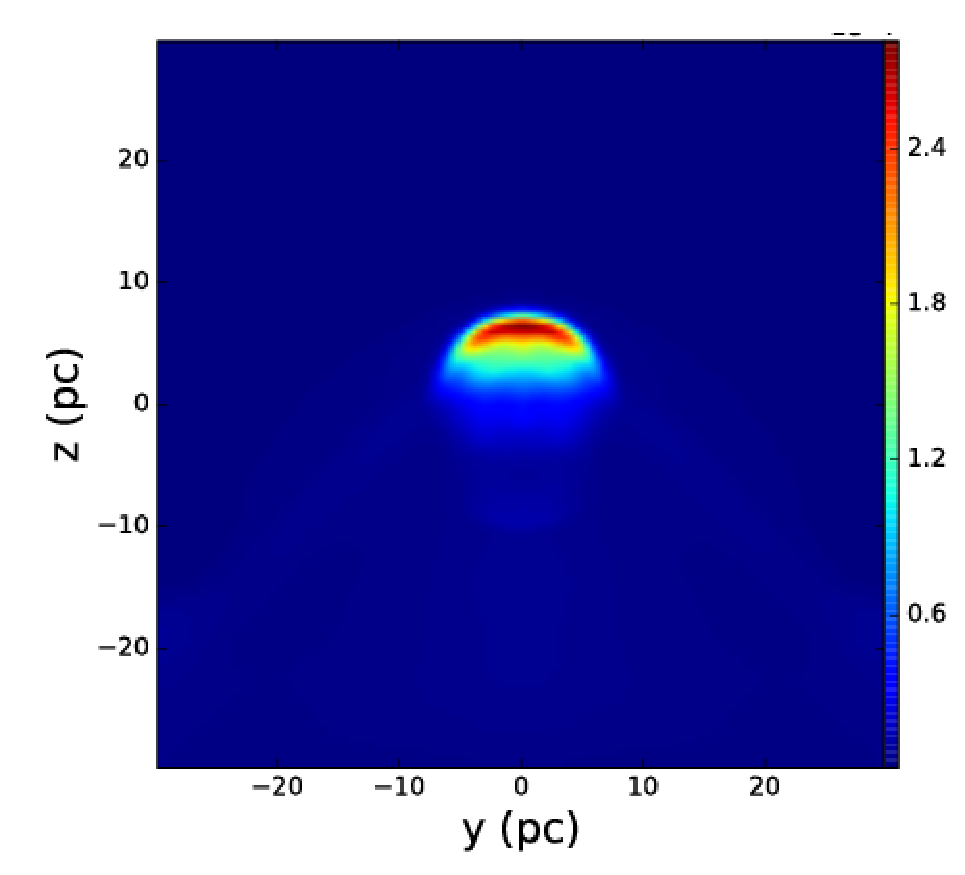
\includegraphics[width=0.325\textwidth]{t6_yzpc.eps}\newline
    \caption{考虑热传导的模拟结果。这些结果对应了图~\ref{fig:per}的上面三列,唯一的不同
    就是考虑了热传导。}
\label{fig:conduction}
\end{figure*}

事实上,\citet{Orlando2007}基于非均匀的初始介质假设也可以模拟出与垂直事例相似的图像,
不过他们无法解释这些非均匀条件的来源。
\citet{vanMarle2010}将星风考虑在内,并进行流体模拟以研究其对遗迹演化的影响,不过因为
没有磁场信息无法获得射电图像。
而且他们也没考虑前身星的运动,而大多数恒星相对周围介质是运动的,所以我们的工作是对之前
工作的一个重要的补充。
事实上,之前有很多对特定遗迹的形态进行探讨的工作,比如\citet{Vigh2011}有研究Tycho超新星
遗迹的非对称性,\citet{Schneiter2006}模拟遗迹3C 400.2的形态并探讨了热传导的影响,而
\citet{Toledo-Roy2014}考虑了前身星的运动和星风之后,很好的解释了Kepler超新星遗迹的形态,
\citet{Toledo-Roy2014a}结合X射线和射电观测,基于MHD模拟研究了SNR G352.7−0.1。
而我们的模拟基于前人的工作,提供了更普适的解释方式。

另一个有趣的事情是,图~\ref{fig:per}第三行中不同图像的相对射电流量密度差距很大。
x-z平面中最低,x-y平面中高一些,y-z平面中最高。
要知道,这三幅图是一个遗迹爆发从不同方向看的结果,所以一个遗迹从不同方向看,流量密度不同,
那能探测到的概率也是不一样的。
换言之,如果只考虑垂直事例,进行观测结果统计时,单边小弧度的遗迹比双边对称遗迹要多,
双边对称的遗迹比单边大弧度遗迹要多。
而其实有其它情况中也会产生双边对称遗迹,所以在这里我们只能推出单边小弧度的遗迹比单边大弧度
遗迹要多,而表~\ref{table:stat}的统计也支持这一推论。
因而,如果银河系中遗迹爆发朝向我们的方向是随机的,那实际上可观测到的单边小弧度和单边大
弧度遗迹数量应该相近,目前的差值是因为观测的灵敏度不够,如果提高灵敏度可以观测到更多单边
大弧度遗迹。
而从图~\ref{fig:per}第三行中可看出,y-z平面的最大流量密度大概是x-z平面的20倍,所以如果
灵敏度提高20倍,那观测到的单边大弧度遗迹数量就与如今观测到的单边小弧度遗迹相近。
这或许可以解释目前观测到的大约300个的银河系遗迹数目\citep{2014BASI...42...47G},远少于
理论预言的至少1000个\citep{Frail1994a,Tammann1994},因为理论计算时并没有考虑观测方向
导致的流量变化。

\begin{figure*}
    \centering
    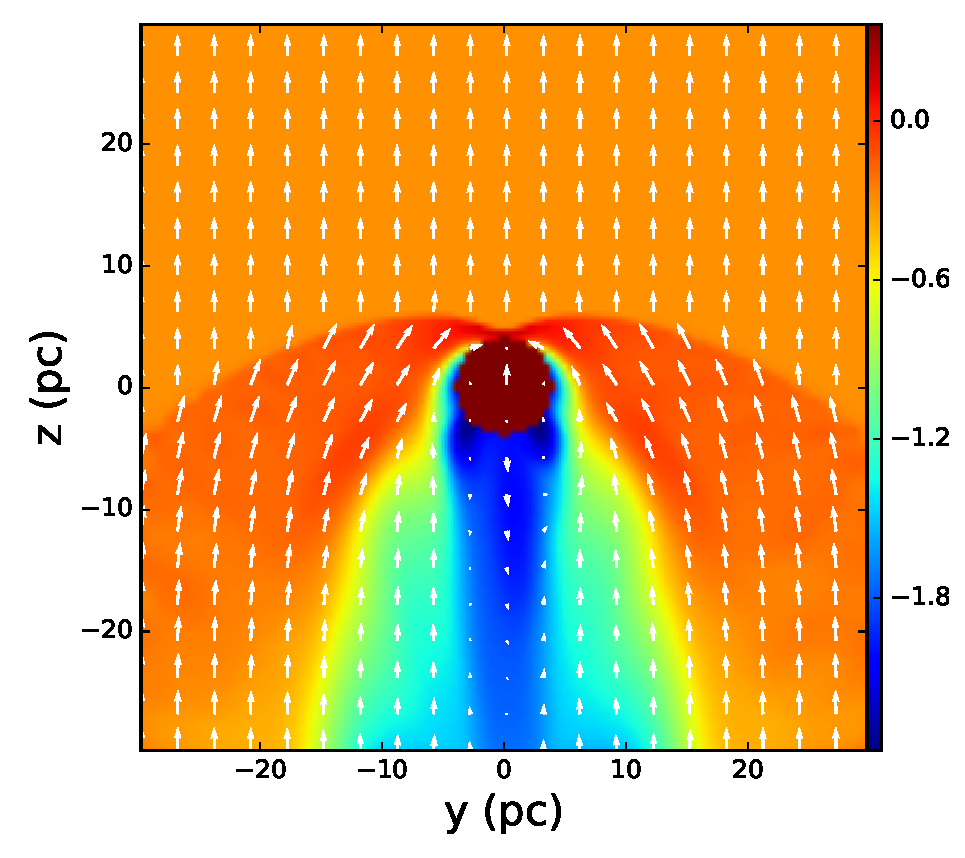
\includegraphics[width=0.325\textwidth]{rho_t0_density1_E1_yz.eps}
    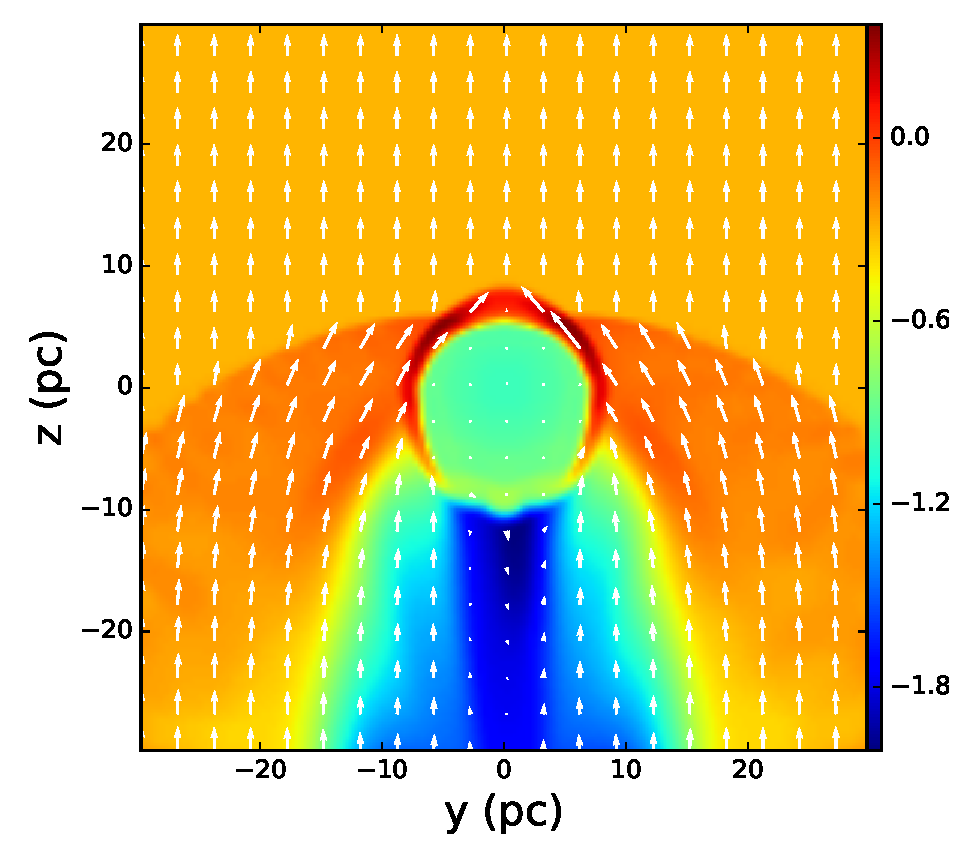
\includegraphics[width=0.325\textwidth]{rho_t6_density1_E1_yz.eps}
    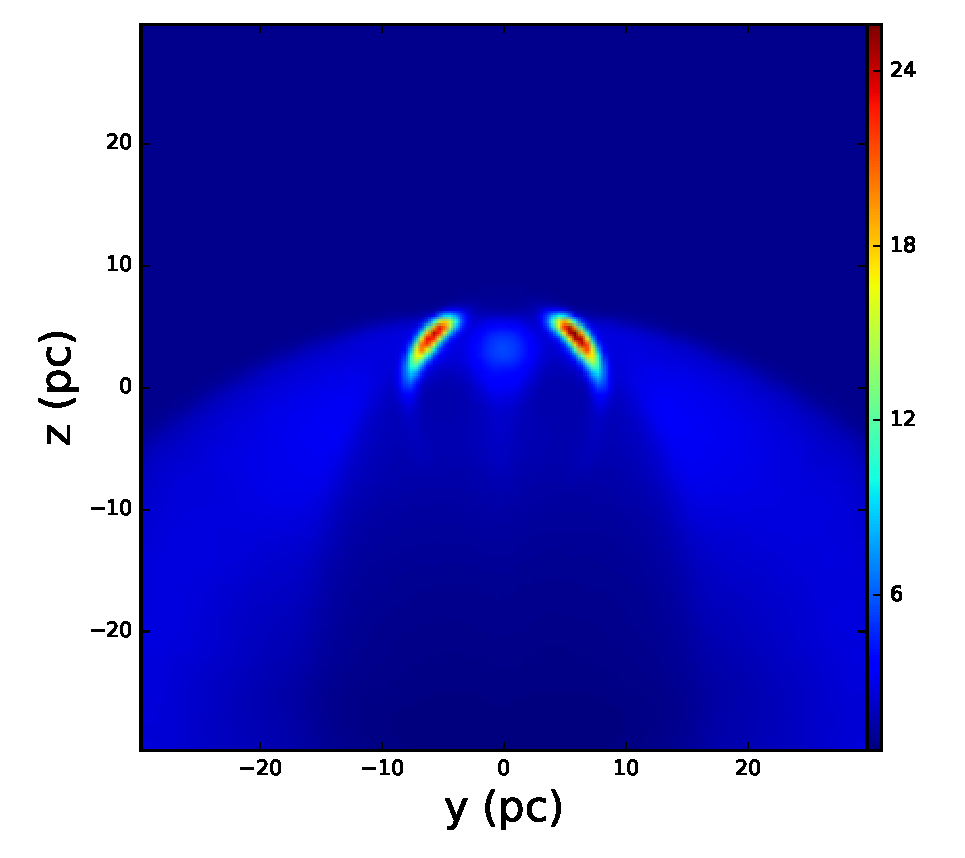
\includegraphics[width=0.325\textwidth]{t6_yz.eps}
    \caption{平行事例的模拟结果。 左图是y-z平面的星风模拟结果加上遗迹爆发区域,也就是
    遗迹模拟的初始条件。中图是y-z平面的遗迹模拟结果。右图是从中图转化来的射电流量密度图。}
\label{fig:par}
\end{figure*}

此外,因为热传导在星风演化中起重要作用,所以我们也在整个遗迹模拟中测试了是否热传导会影响
遗迹的射电形态。
我们使用了模拟软件PLUTO中的Explicit框架,采取标准热传导系数计算方式。
图~\ref{fig:conduction}是最终的模拟结果,从整体图像可以看出与不考虑热传导相比,本来就
有的弓形壳层变成了两层,而磁场也变得明显不同。
\citet{Meyer2015}提到热传导会引起物质混合的效应,不过在我们的模拟中并不明显,可能是因为
我们用的遗迹模拟参数不同。
不过在超新星遗迹周围,密度和磁场并没有明显的变化。
相应的,遗迹周围的射电图像与图~\ref{fig:per}几乎完全一样,而其他位置即使有射电图像,因为
那里应该没有相对论化电子,同步辐射假设不成立,因而也就没有意义。
总而言之,热传导对超新星遗迹的射电演化影响不大。

\subsection{平行事例}



\begin{figure*}
    \centering
    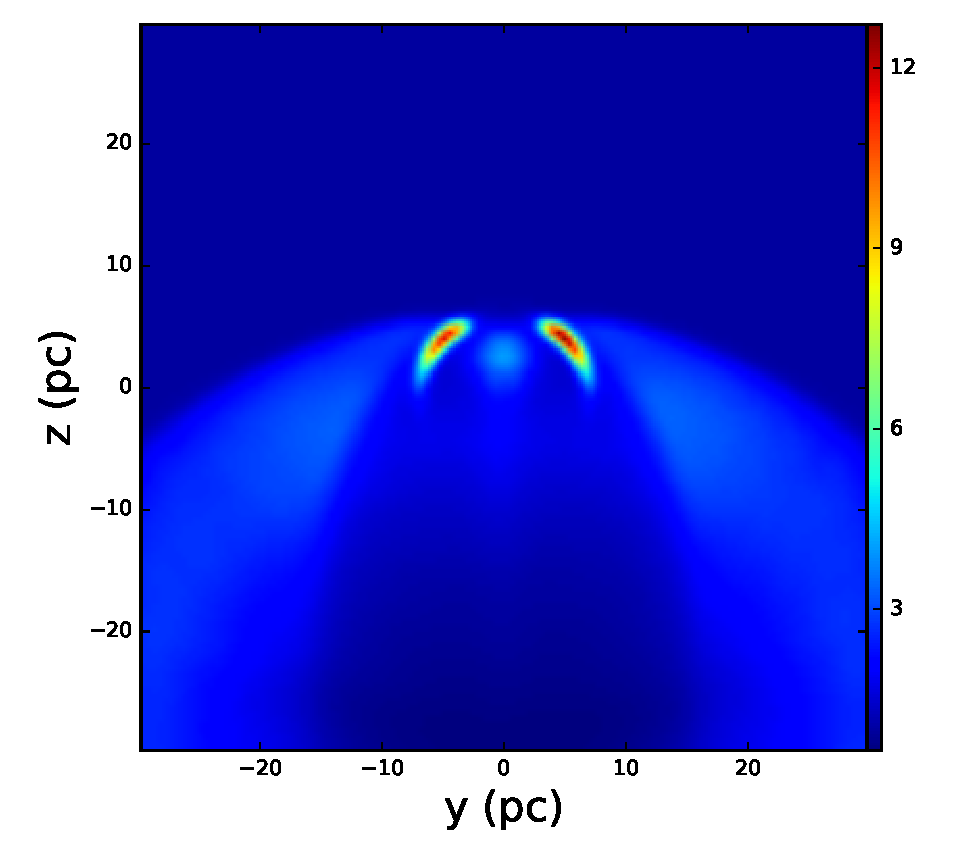
\includegraphics[width=0.325\textwidth]{t4_yz.eps}
    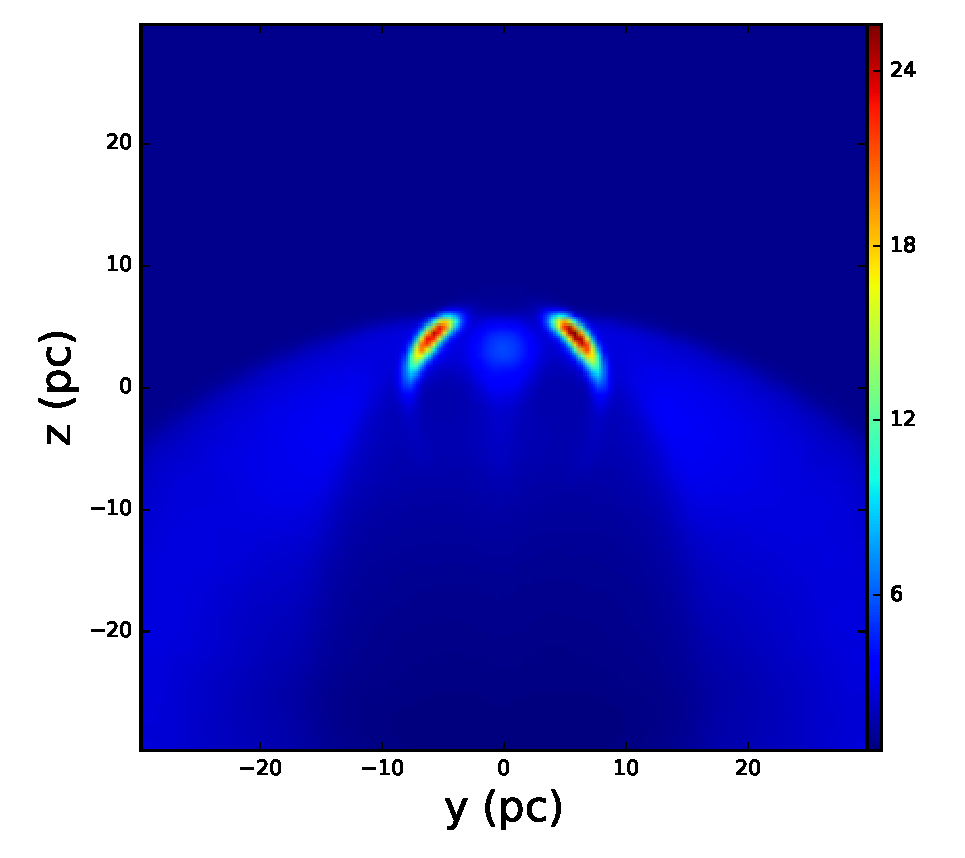
\includegraphics[width=0.325\textwidth]{t6_yz.eps}
    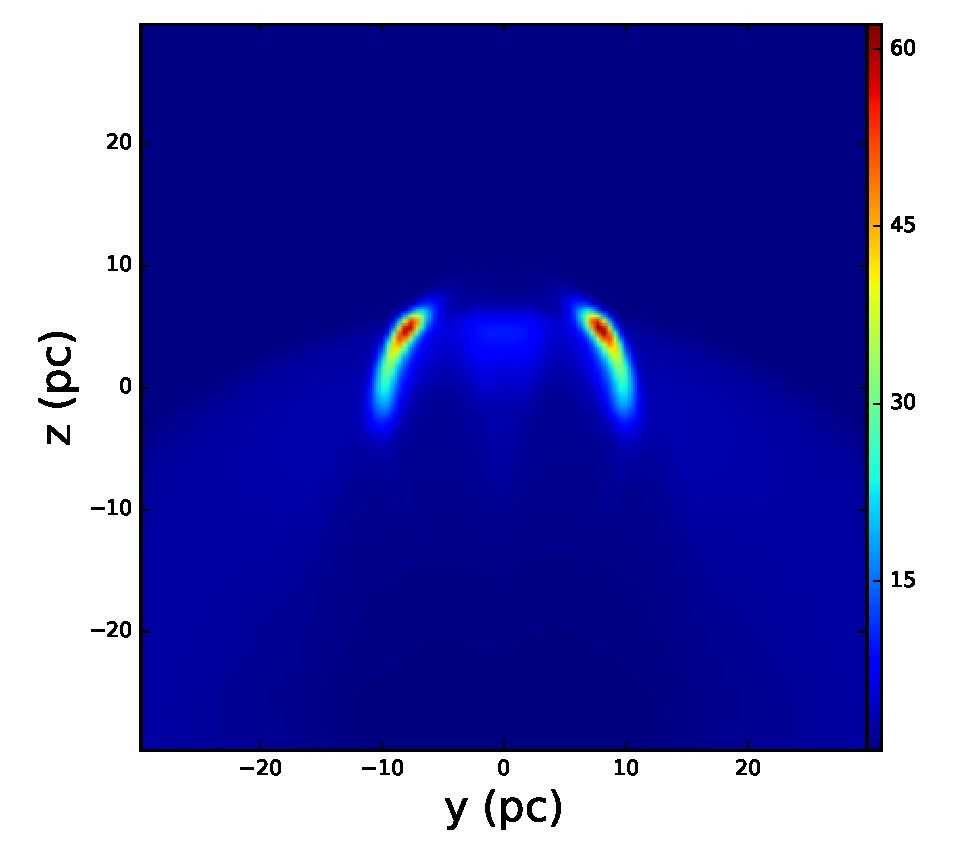
\includegraphics[width=0.325\textwidth]{t12_yz.eps}\newline
    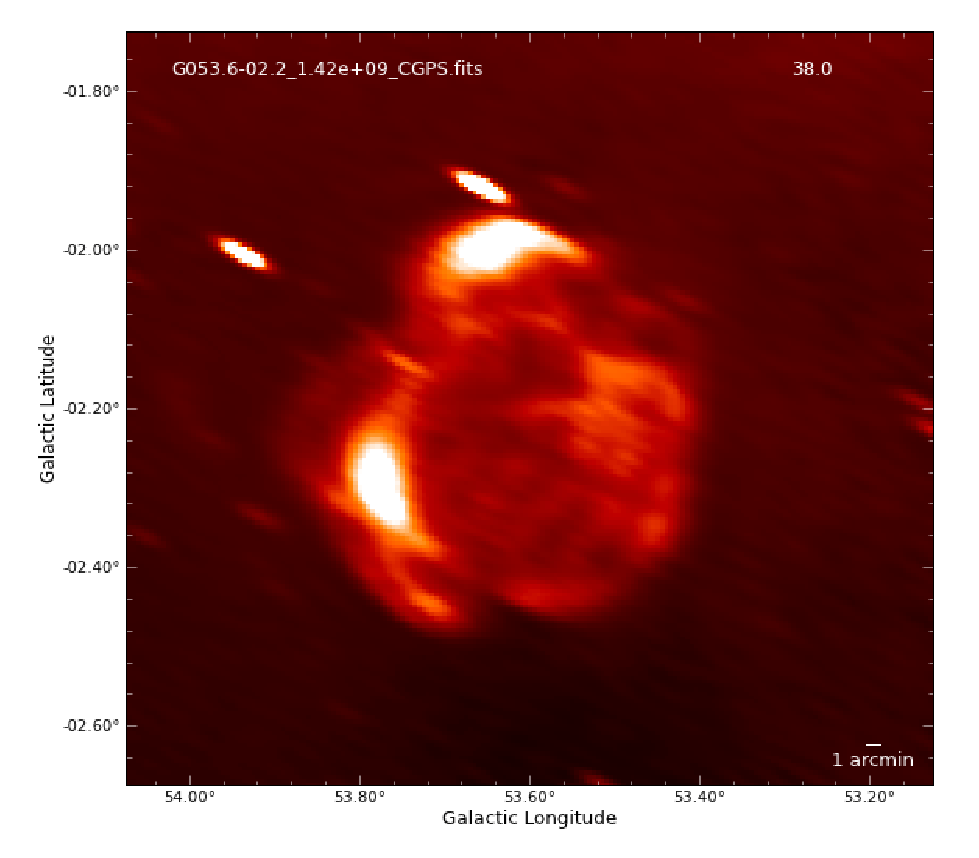
\includegraphics[width=0.325\textwidth]{G53.eps}
    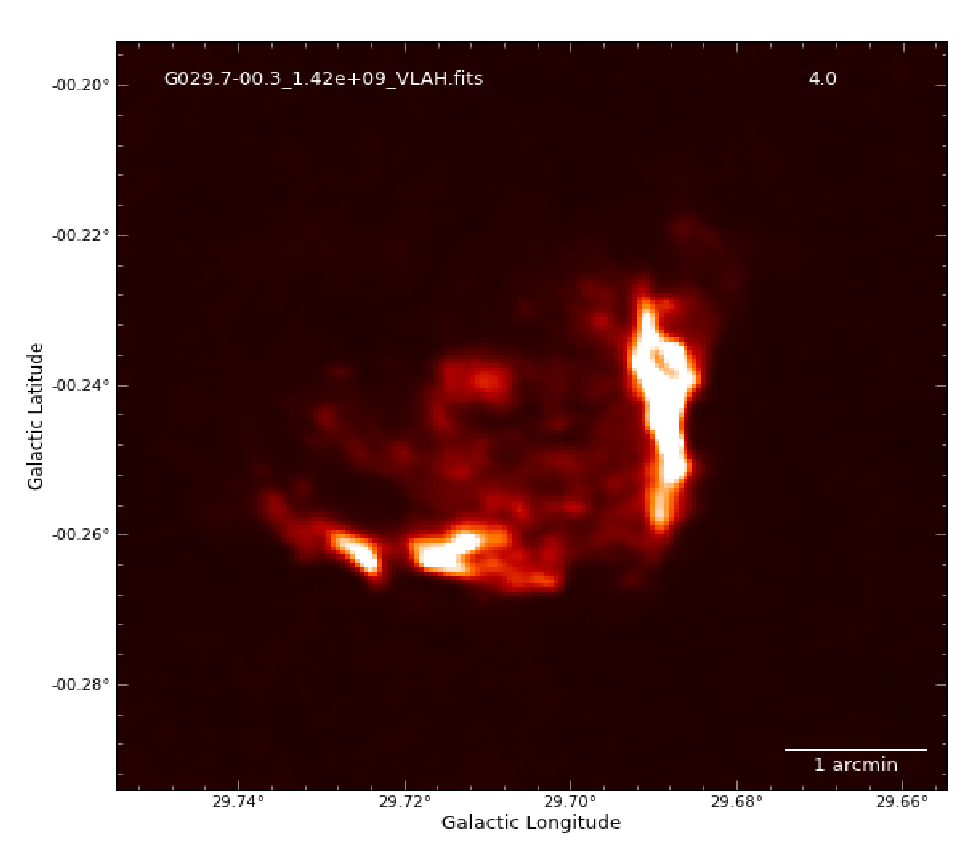
\includegraphics[width=0.325\textwidth]{G29.eps}
    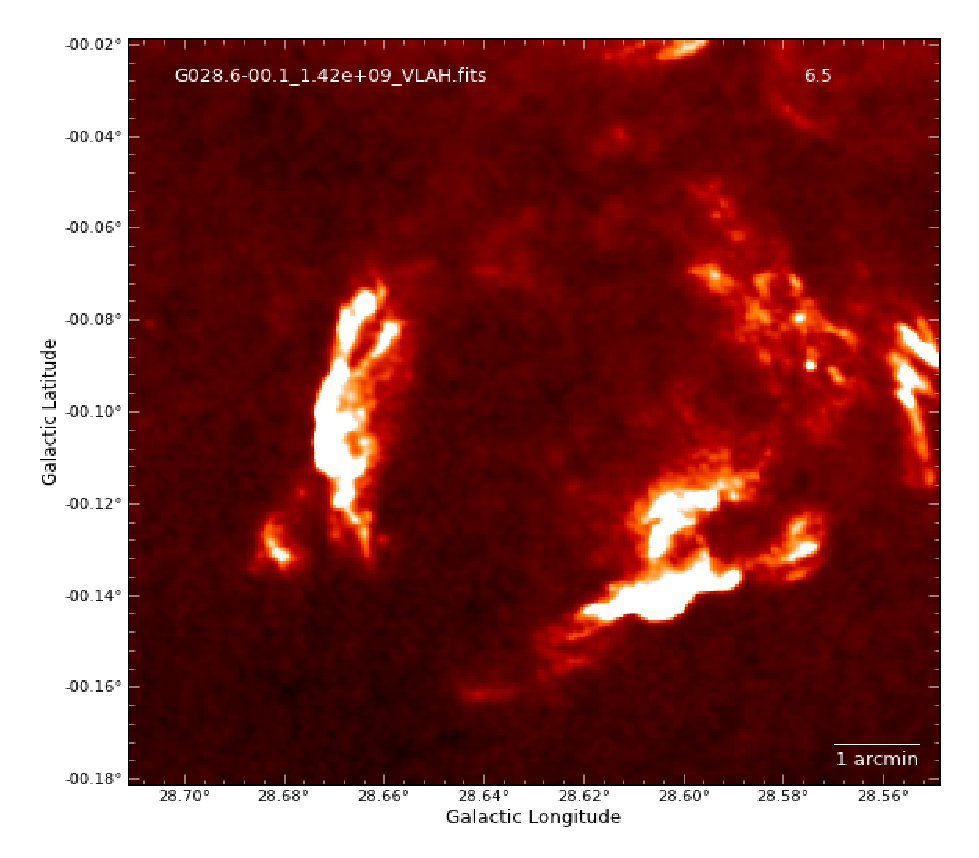
\includegraphics[width=0.325\textwidth]{G28.eps}
    \caption{上面三幅图是不同年龄的相对射电流量密度图。下面三幅图是实际观测到的与上图
    类似的实际观测到的八字形遗迹:G53.6-2.2、G29.7-0.3、G28.6-0.1\citep{West2016}。}
\label{fig:parc}
\end{figure*}

平行事例的结果在图~\ref{fig:par}中,除了磁场方向从沿着y轴变为z轴,其它参数都与垂直事例
完全一样。
要注意的是,虽然除了遗迹周围,其他位置也有辐射,但那是星风模拟导致的,而星风并不能产生
足量相对论电子,因而在那些区域同步辐射假设不成立,因而其辐射是无意义的。
可是,我们也无法剔除这些无意义的结构,因为我们不清楚相对论电子所能影响到的范围。
这个瑕疵其实也影响到垂直事例,只是不够明显。
我们只在图~\ref{fig:par}中展示了y-z平面的结果,因为磁场方向和前身星速度方向一直,多了
对称性,整个演化为柱对称,x-y平面与y-z平面演化是一样的。
此外,理论上在x-y平面我们应该看到环形遗迹,可实际上看到的却很方,这是因为分辨率不够高,
而每一个像素点是方形的。
超新星爆发能量又很大,这会导致局部变量变化很快,要更好模拟需要很高分辨率才行,而在我们的
工作集群上使用能达到的分辨率上限也无法完美模拟出环形,因而我们只能说,理论上看,x-y平面
肯定能看到一个环形遗迹。

所以,从图~\ref{fig:par}看来,平行事例给我们展示的只有一个新的形态:八字形遗迹。
但是这个形态其实非常重要,因为之前的模拟都很难解释这个形态,而这一类的遗迹其实并不少。
所以,如果把理论上肯定存在的环形超新星遗迹考虑在内,我们总共可以模拟出五类超新星遗迹,
只有多层和不规则遗迹无法解释。
这两类遗迹可能的确是因为初始的周围介质是不均匀或者前身星比较奇特
\citep{Orlando2007,Orlando2017}。

目前为止,我们提到的模拟都是1850年演化之后的结果,而实际上我们可以给出任何时间的结果,
只要不是太长以至于超过计算集群的运行极限。
所以我们在图~\ref{fig:parc}给出了模拟1450年、1850年和3050年后的平行事例结果,作为比较,
同时给出了三个形状相似的真实观测到的八字形遗迹:G53.6-2.2、G29.7-0.3、G28.6-0.1。
那么很自然的,我们猜测是否这三个遗迹年龄都在几千年左右。
实际上,G29.7-0.3是1000年左右\citep{Leahy2008},G28.6-0.1不超过2700年\citep{Bamba2001},
与我们估计相符。
可是G53.6-2.2年龄估计为15000年\citet{Long1991},不过其年龄估计所用的距离很可能有问题,
需要进一步验证。
除此之外,这三个遗迹的X射线辐射都多少偏离射电辐射\citep{Broersen2015,Su2009,Bamba2001},
类似于超新星遗迹G116.9+0.2,这也可以用类似的方式解释。

同时,因为我们在垂直事例和平行事例中用的参数基本一样,我们可以直接比较两个事例的模拟结果。
比较图~\ref{fig:par}和图~\ref{fig:per}可知,平行事例在y-z平面的相对射电流量比垂直事例
的大很多。
也就是说,八字形遗迹应该比单边小弧度遗迹要少,这也是与表~\ref{table:stat}的统计一直。
同时,看x-z平面的话,单边大弧度遗迹应该比八字形遗迹要少,这却与表~\ref{table:stat}的统计
相反,单边大弧度遗迹反而比八字形遗迹要多一点。
这可能因为两者本来模拟的流量密度相差不大,而样本量又少,从而导致的统计偏差。

\section{总结}
\label{SWsum}
我们将星风演化结果作为超新星遗迹模拟的初始条件,模拟了一个以40 \kms 运动的40 M$_{\odot}$
前身星爆发后的遗迹演化。
整个工作包括了两个模拟:垂直事例和平行事例。
基于真实的射电图像,我们将超新星遗迹分为七类,并以此结合模拟结果做了进一步讨论。
我们主要的结论如下:

\begin{enumerate}

    \item 大质量前身星的星风对超新星遗迹的射电形态有很大影响,可能比最初的周围环境影响
    还大。

    \item 将星风考虑在内,我们可以解释很多遗迹的射电形态,除了多层和不规则遗迹。

    \item 根据模拟结果,我们不建议通过超新星遗迹的射电图像推测大尺度的磁场和密度分布。

    \item 热传导或许会稍微影响遗迹的射电形态,但是并不是非常重要。

    \item 某些遗迹的射线壳层与X射线辐射的偏离可能是因为前身星的运动。

\end{enumerate}

在此,需要提醒的是,我们的工作中有很多简化,讨论时需要注意。
而我们模拟的40 M$_{\odot}$太阳质量前身星其实并不是非常普遍,所以将来可以尝试做
10$\sim$20 M$_{\odot}$的模拟。
此外,多层遗迹的形成原因也是一个有趣的研究方向,我们将在章节~\ref{Mag}中尝试用强磁场解释
这件事情。
